% $Header: /home/vedranm/bitbucket/beamer/solutions/generic-talks/generic-ornate-15min-45min.en.tex,v 90e850259b8b 2007/01/28 20:48:30 tantau $

\documentclass{beamer}

% This file is a solution template for:

% - Giving a talk on some subject.
% - The talk is between 15min and 45min long.
% - Style is ornate.



% Copyright 2004 by Till Tantau <tantau@users.sourceforge.net>.
%
% In principle, this file can be redistributed and/or modified under
% the terms of the GNU Public License, version 2.
%
% However, this file is supposed to be a template to be modified
% for your own needs. For this reason, if you use this file as a
% template and not specifically distribute it as part of a another
% package/program, I grant the extra permission to freely copy and
% modify this file as you see fit and even to delete this copyright
% notice.


\mode<presentation>
{
  \usetheme{Warsaw}
  % or ...

  \setbeamercovered{transparent}
  % or whatever (possibly just delete it)
}

      \theoremstyle{theorem}
      \newtheorem{proposition}[theorem]{Proposition}
      \theoremstyle{definition}
      \newtheorem{game}[theorem]{Game}
      \newtheorem{question}[theorem]{Question}

\usepackage[english]{babel}
% or whatever

\usepackage[latin1]{inputenc}
% or whatever

\usepackage{times}
\usepackage[T1]{fontenc}
% Or whatever. Note that the encoding and the font should match. If T1
% does not look nice, try deleting the line with the fontenc.


\usepackage{marvosym} % For \Smiley
\usepackage{verbatim} % for \verbatiminput

\title
{The Math of Games}

\subtitle
{at Huntingdon College} % (optional)

\author%[Author, Another] % (optional, use only with lots of authors)
{Steven~Clontz~\\http://stevenclontz.com}%\inst{1} \and S.~Another\inst{2}}
% - Use the \inst{?} command only if the authors have different
%   affiliation.

\institute[Auburn University] % (optional, but mostly needed)
{
  %\inst{1}%
  Department of Mathematics and Statistics\\
  Auburn University}
  %\and
  %\inst{2}%
  %Department of Theoretical Philosophy\\
  %University of Elsewhere}
% - Use the \inst command only if there are several affiliations.
% - Keep it simple, no one is interested in your street address.

\date[14-06-23] % (optional)
{June 23, 2014}


% If you have a file called "university-logo-filename.xxx", where xxx
% is a graphic format that can be processed by latex or pdflatex,
% resp., then you can add a logo as follows:

 % \pgfdeclareimage[height=1cm]{university-logo}{auburn_logo.png}
 % \logo{\pgfuseimage{university-logo}}



% Delete this, if you do not want the table of contents to pop up at
% the beginning of each subsection:
%\AtBeginSubsection[]
%{
%  \begin{frame}<beamer>{Outline}
%    \tableofcontents[currentsection,currentsubsection]
%  \end{frame}
%}


% If you wish to uncover everything in a step-wise fashion, uncomment
% the following command:

%\beamerdefaultoverlayspecification{<+->}

% My game notational definitions
\newcommand{\win}{\uparrow}
\newcommand{\prewin}{\uparrow_{\text{pre}}}
\newcommand{\markwin}{\uparrow_{\text{mark}}}
\newcommand{\tactwin}{\uparrow_{\text{tact}}}
\newcommand{\ktactwin}[1]{\uparrow_{#1\text{-tact}}}
\newcommand{\kmarkwin}[1]{\uparrow_{#1\text{-mark}}}
\newcommand{\codewin}{\uparrow_{\text{code}}}
\newcommand{\limitwin}{\uparrow_{\text{limit}}}
\newcommand{\oneptcomp}[1]{#1^*}
\newcommand{\oneptlind}[1]{#1^\dagger}
\newcommand{\congame}[2]{Con_{\pl O\pl P}(#1,#2)}
\newcommand{\clusgame}[2]{Clus_{\pl O\pl P}(#1,#2)}
\newcommand{\lfkpgame}[1]{LF_{\pl K\pl P}(#1)}
\newcommand{\lfklgame}[1]{LF_{\pl K\pl L}(#1)}
\newcommand{\pfgame}[1]{PF_{\pl F\pl C}(#1)}
\newcommand{\mengame}[1]{Cov_{\pl C\pl F}(#1)}
\newcommand{\rothgame}[1]{Cov_{\pl C\pl S}(#1)}
\newcommand{\altrothgame}[1]{Cov_{\pl P\pl O}(#1)}
\newcommand{\fillgame}[1]{Fill^{\subseteq}_{\pl M\pl N}(#1)}
\newcommand{\sfillgame}[1]{Fill^{\subsetneq}_{\pl M\pl N}(#1)}
\newcommand{\kfillgame}[1]{Fill^{\subseteq}_{\pl C\pl F}(#1)}
\newcommand{\ksfillgame}[1]{Fill^{\subsetneq}_{\pl C\pl F}(#1)}
\newcommand{\recallgame}[2]{Rec^{#1}_{\pl F\pl S}(#2)}
\newcommand{\sigmaprodr}[1]{\Sigma\mathbb{R}^{#1}}
\newcommand{\sigmaprodtwo}[1]{\Sigma2^{#1}}
\newcommand{\concat}{^\frown}
\newcommand{\rest}{\restriction}
\newcommand{\cl}[1]{\overline{#1}}
\newcommand{\pow}[1]{\mc{P}(#1)}
\newcommand{\<}{\langle}
\renewcommand{\>}{\rangle}
\newcommand{\al}[1]{{#1}^*}
\newcommand{\mc}[1]{\mathcal{#1}}
\newcommand{\po}{\mathbb{P}}
\newcommand{\pok}{\po_\kappa}
\newcommand{\Lim}{\mathrm{Lim}}
\newcommand{\Suc}{\mathrm{Suc}}
\newcommand{\ds}{\displaystyle}
\newcommand{\alcomp}{\al\parallel}
\newcommand{\rank}{\textrm{rank}}
\newcommand{\dom}{\textrm{dom}}
\newcommand{\scish}{almost-$\sigma$-(relatively compact)}

\usepackage{mathrsfs}
\newcommand{\pl}[1]{\mathscr{#1}}

\newcommand{\vpause}{\pause\vspace{1em}}

\newcommand{\term}[1]{\textbf{#1}}




\begin{document}
\renewcommand{\pause}{}

\begin{frame}
  \titlepage
\end{frame}

% \begin{frame}{Table of Contents}
%   \tableofcontents
%   % You might wish to add the option [pausesections]
% \end{frame}

\section{Introduction}

\subsection{Abstract}

\begin{frame}{Abstract}%{Subtitles are optional.}
    \small
    Two player games of perfect information such as chess and checkers have
    been played for centuries. Such games can be analyzed using tools from
    the field of game theory.

    \vpause

    We will define two simple games: Takeaway and Nim.
    Using game theory, we will show how to create a \term{winning strategy}
    for one of the players in each game.

    \vpause

    Also, we will show how \textit{any} game can be analyzed in order
    to produce a winning strategy (given enough computational power).
\end{frame}

\subsection{What's Game Theory?}

\begin{frame}{About game theory}
  Game theory is a broad subject, but in any context, it typically involves the
  mathematics of decision making.

  \vpause

  Economists use game theory to study \term{two-player simultaneous}
  games. Suppose two companies have to set a price on competiting products.
  The demand for each product depends on the decisions made by both companies

  \vpause

  Another example would be \term{games of chance} like Solitaire or Yahtzee.
  One or more players use dice rolls or a shuffled deck of cards to play such
  games, and have to use probability to make decisions based upon future rolls
  of the dice or face-down cards.
\end{frame}

\begin{frame}{Two-player Sequential Games}
  We'll be talking about \term{two-player sequential} games today. These are
  games of \term{perfect information}: the players take turns with full
  knowledge of the history of their opponent's moves.

  \vspace{1em}

  % great example is chess, white and black take turns making moves, which
  % are recorded.

  \centerline{
    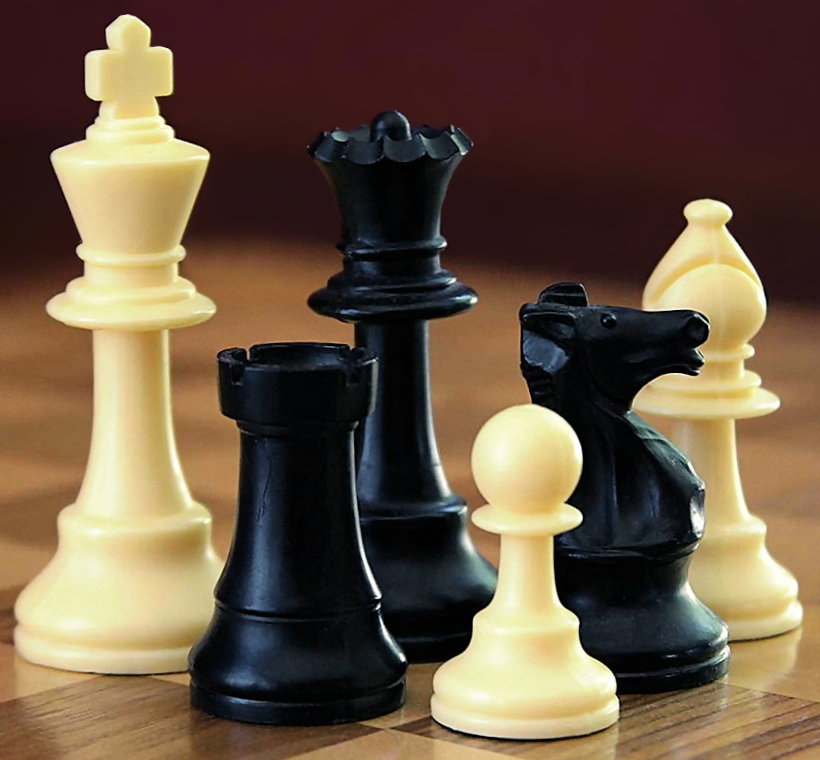
\includegraphics[height=1.5in]{chessPieces.jpg}
    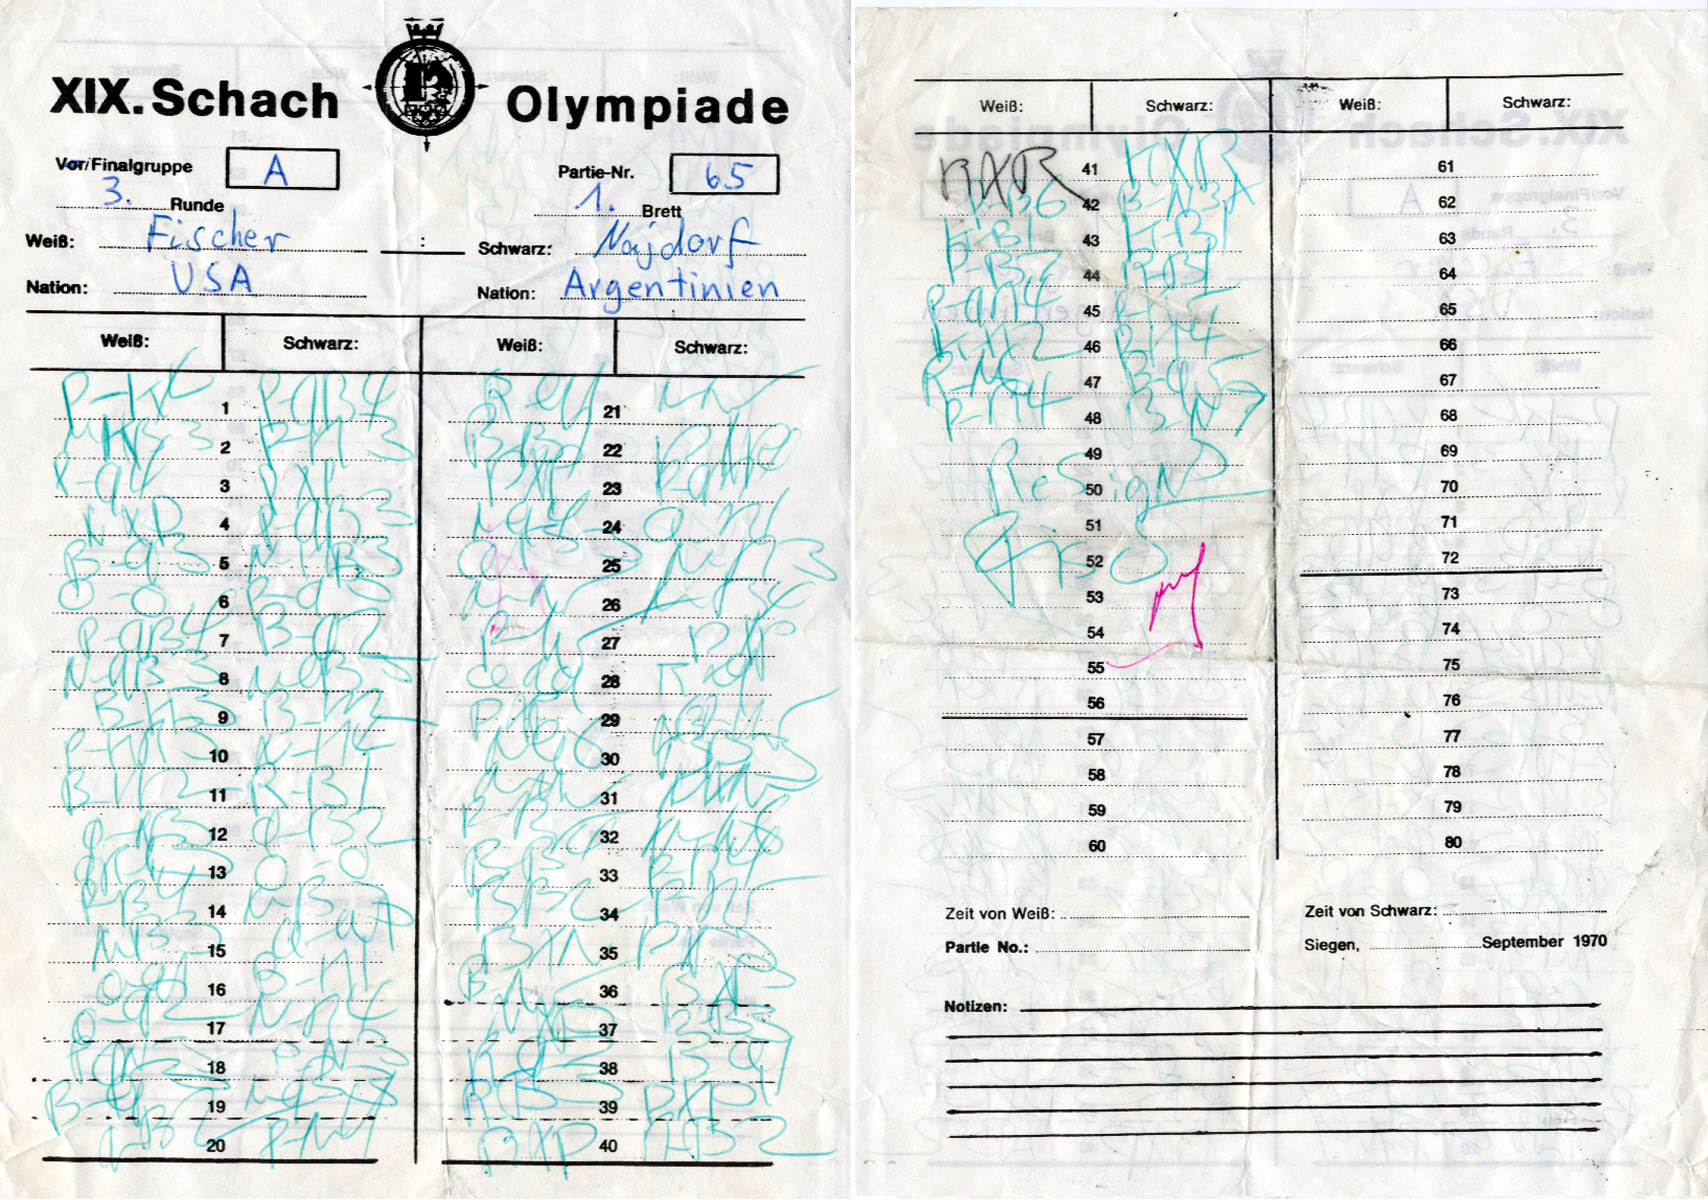
\includegraphics[height=1.5in]{chessNotation.jpg}
  }
\end{frame}

\section{A Couple of Basic Games}

\begin{frame}{Coin games}
  The two games we'll talk about are \term{coin games}, because they can be
  played with whatever loose change you have in your pocket.

  \centerline{
    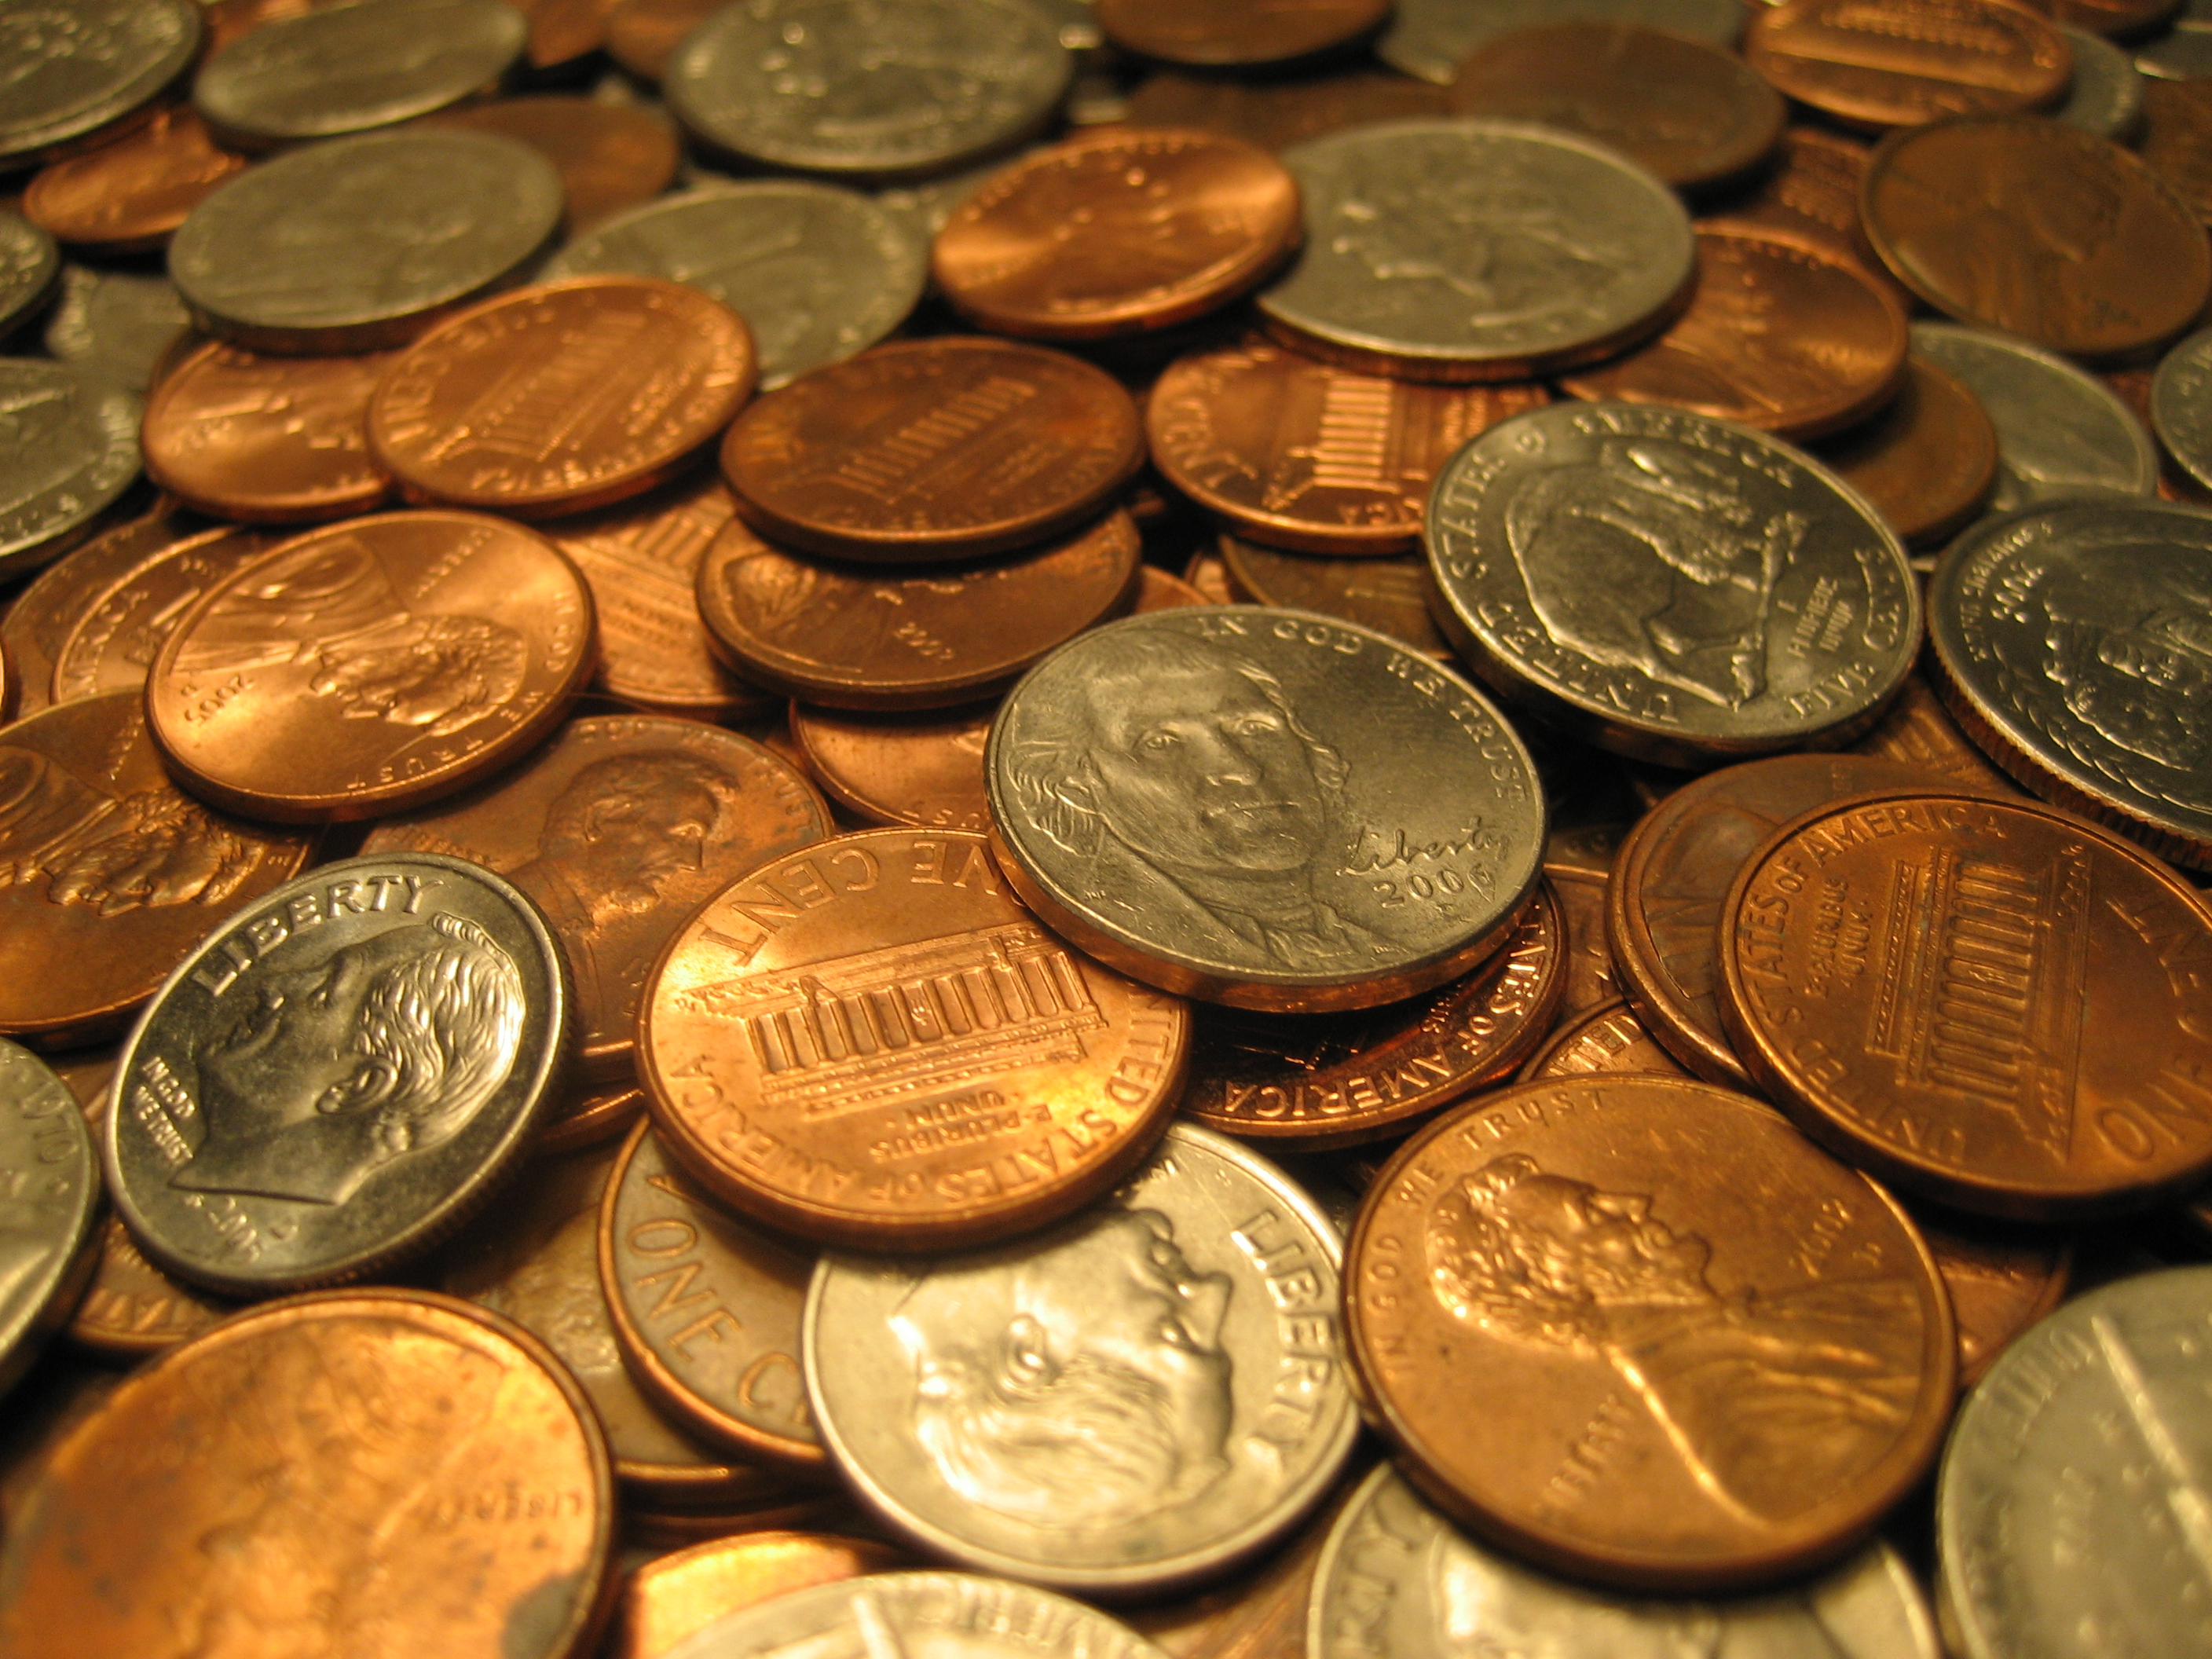
\includegraphics[height=2in]{coins.jpg}
  }
\end{frame}

\subsection{Takeaway}

\begin{frame}{Takeaway}
  In \term{Takeaway}, the Players $\pl A$, $\pl B$ take turns removing $1$,
  $2$, or $3$ coins from a pile (with $15$ coins perhaps). The player who
  removes the last coin wins.

  \vspace{1em}

  \centerline{
    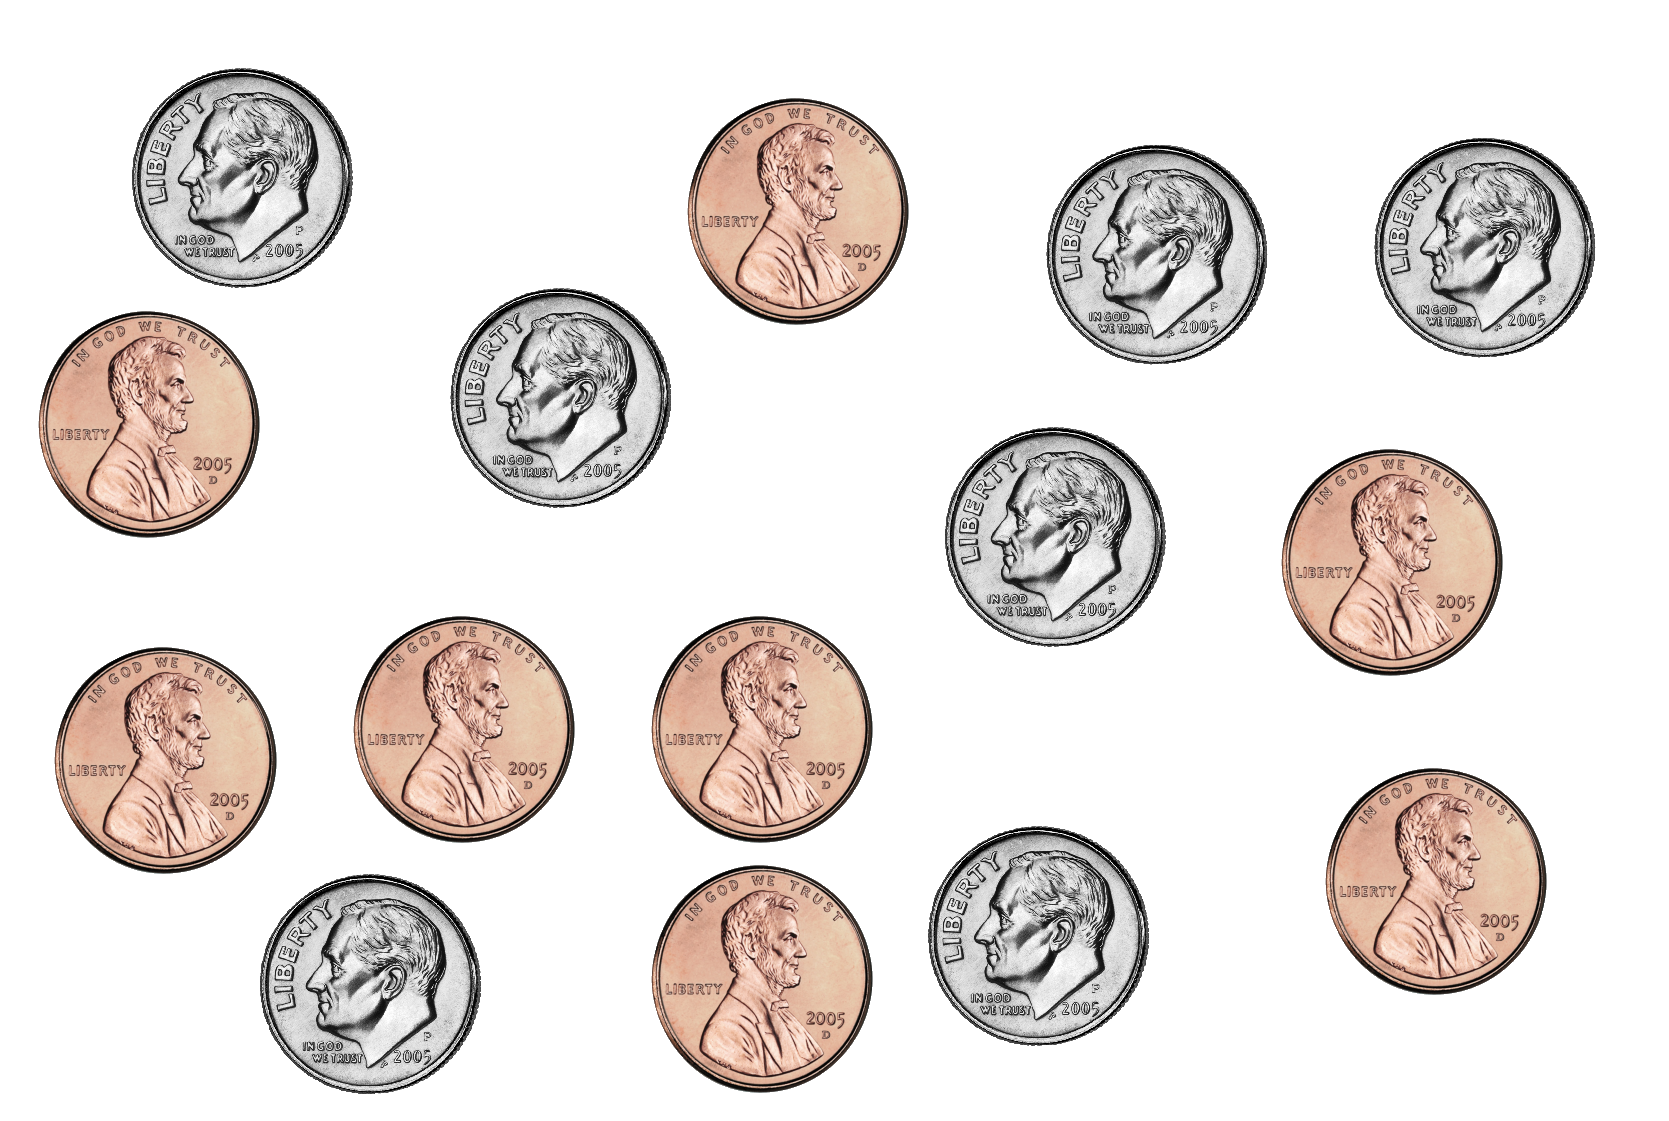
\includegraphics[height=1.7in]{takeawayCoins/15.pdf}
  }
\end{frame}

\begin{frame}
  Round 1a: Player $\pl A$ takes away 3 coins, leaving 12.

  \centerline{
    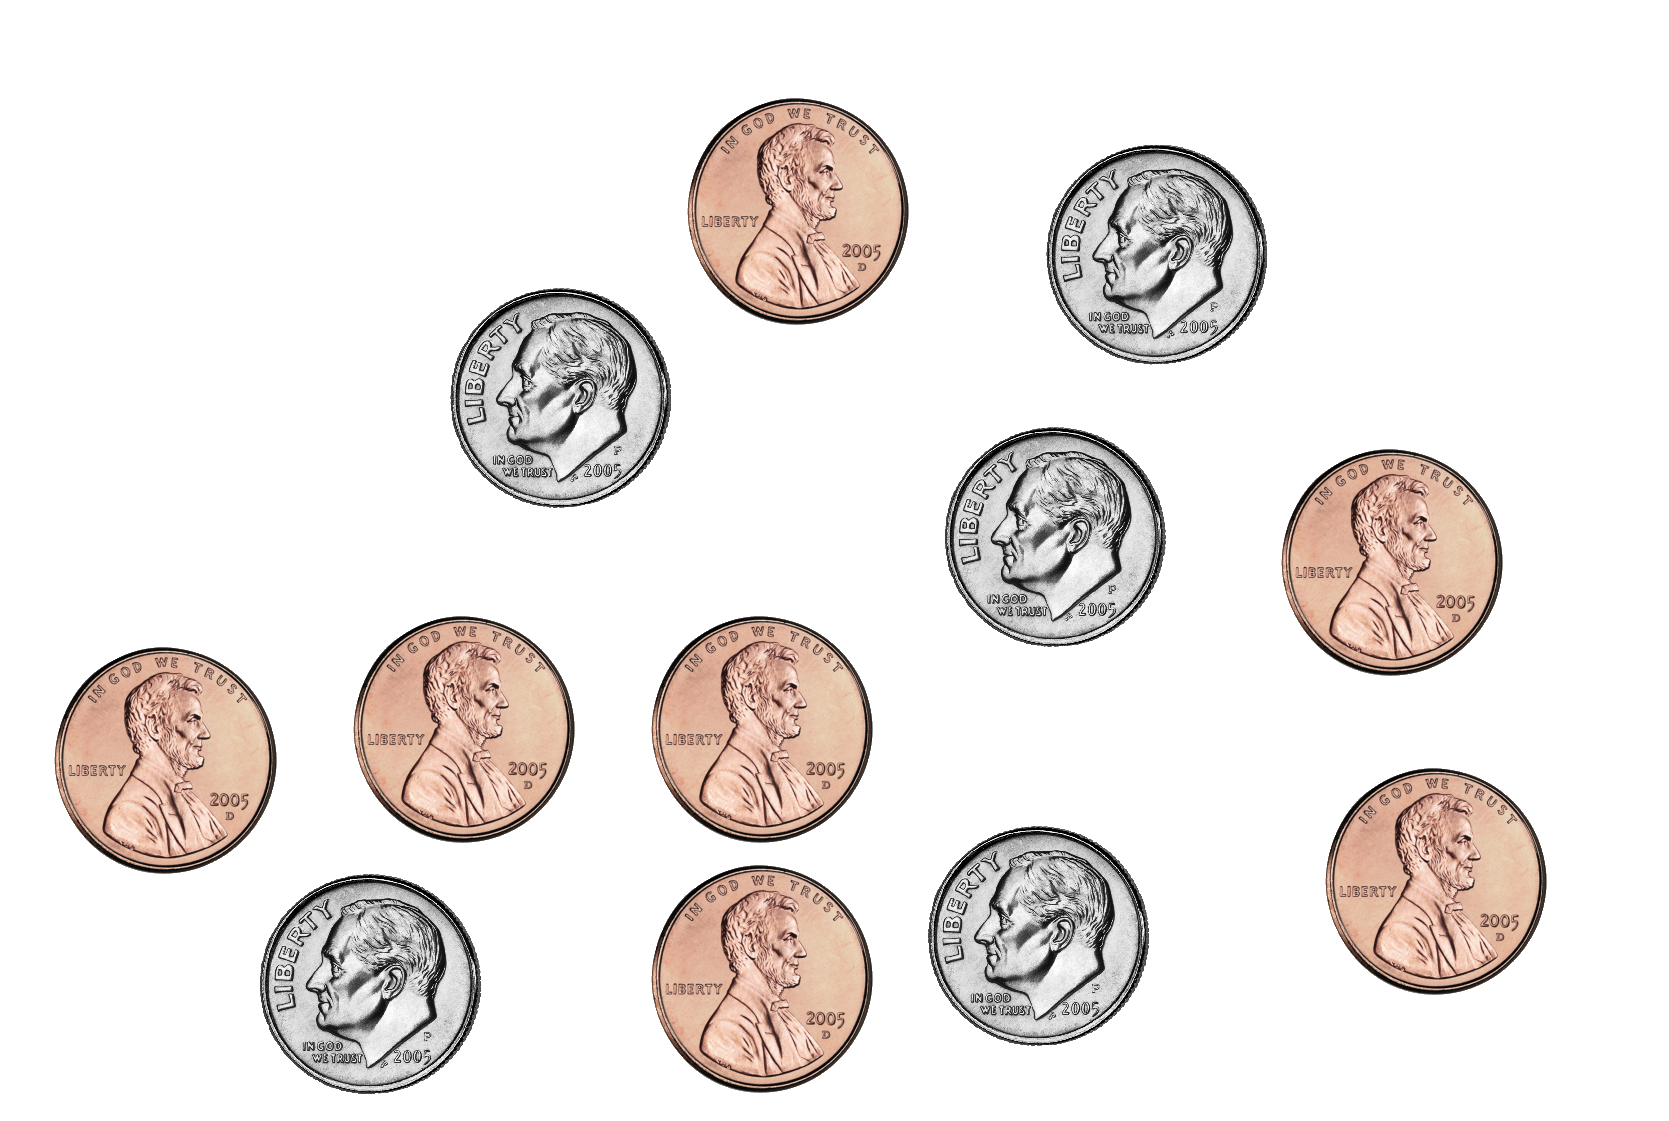
\includegraphics[height=1.7in]{takeawayCoins/12.pdf}
  }
\end{frame}

\begin{frame}
  Round 1b: Player $\pl B$ takes away 2 coins, leaving 10.

  \centerline{
    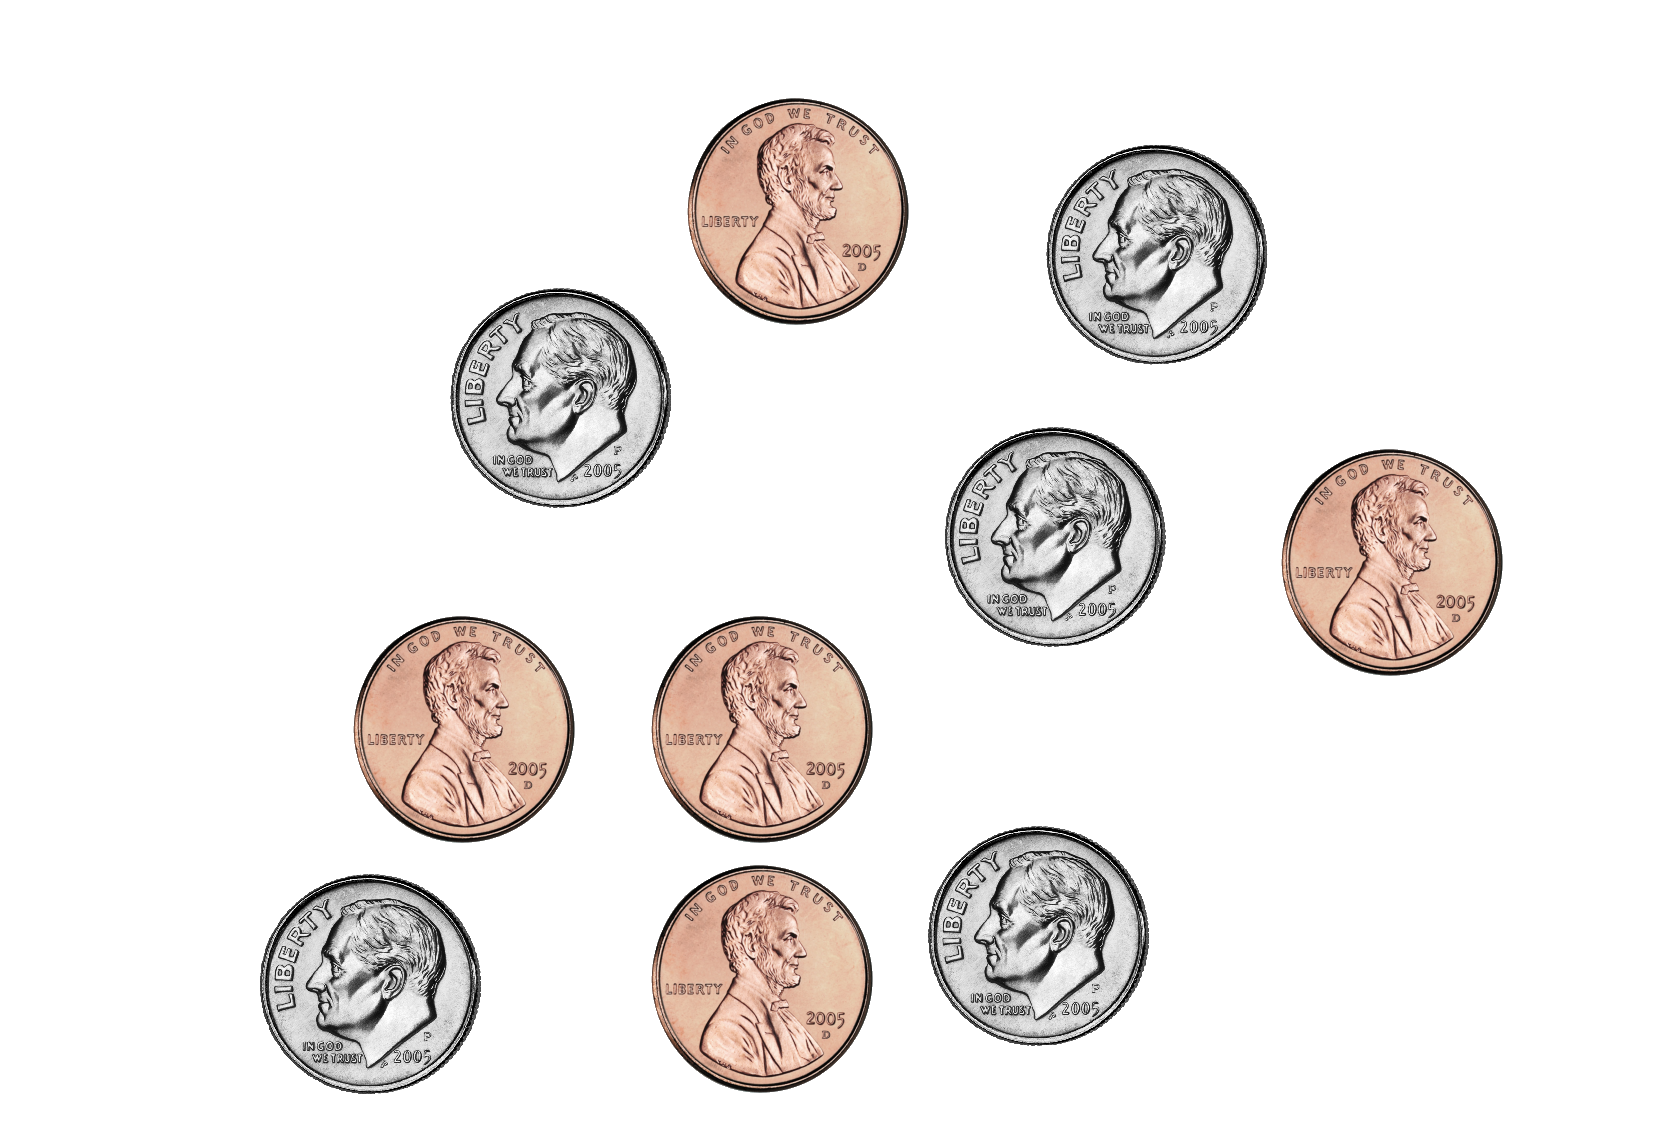
\includegraphics[height=1.7in]{takeawayCoins/10.pdf}
  }
\end{frame}

\begin{frame}
  Round 2a: Player $\pl A$ takes away 1 coin, leaving 9.

  \centerline{
    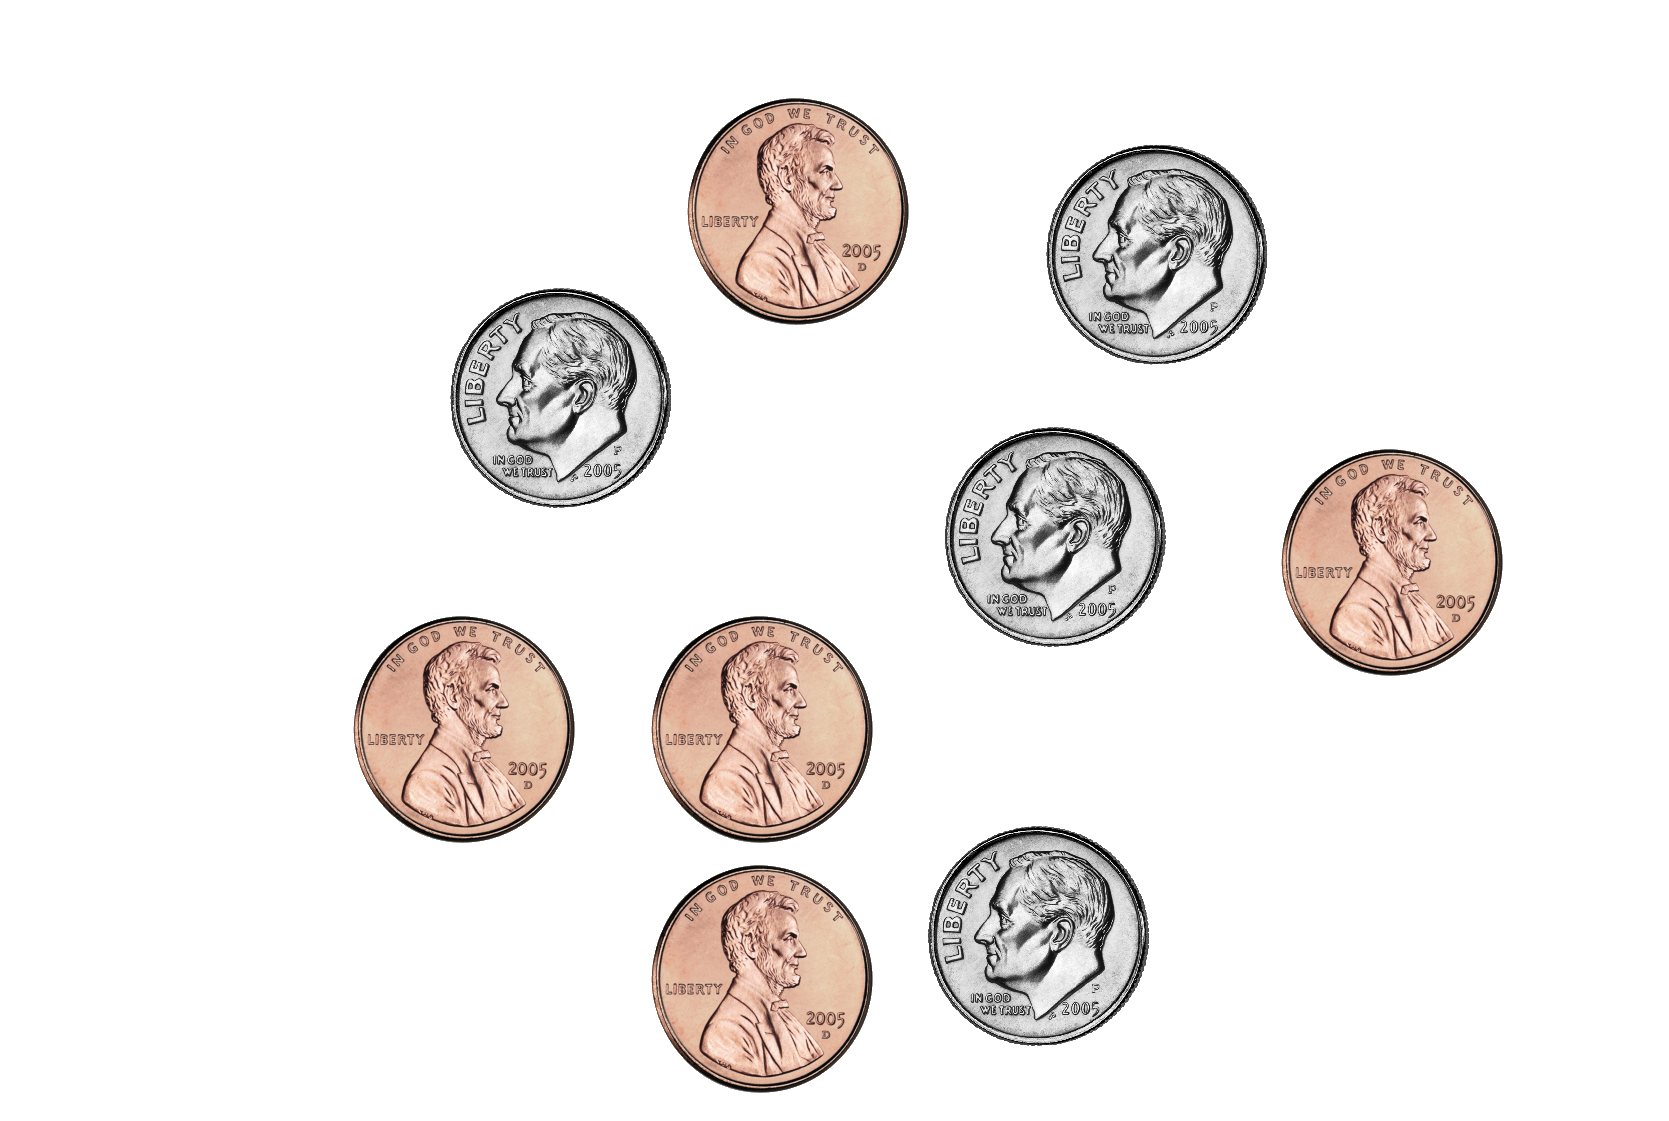
\includegraphics[height=1.7in]{takeawayCoins/09.pdf}
  }
\end{frame}

\begin{frame}
  Round 2b: Player $\pl B$ takes away 2 coins, leaving 7.

  \centerline{
    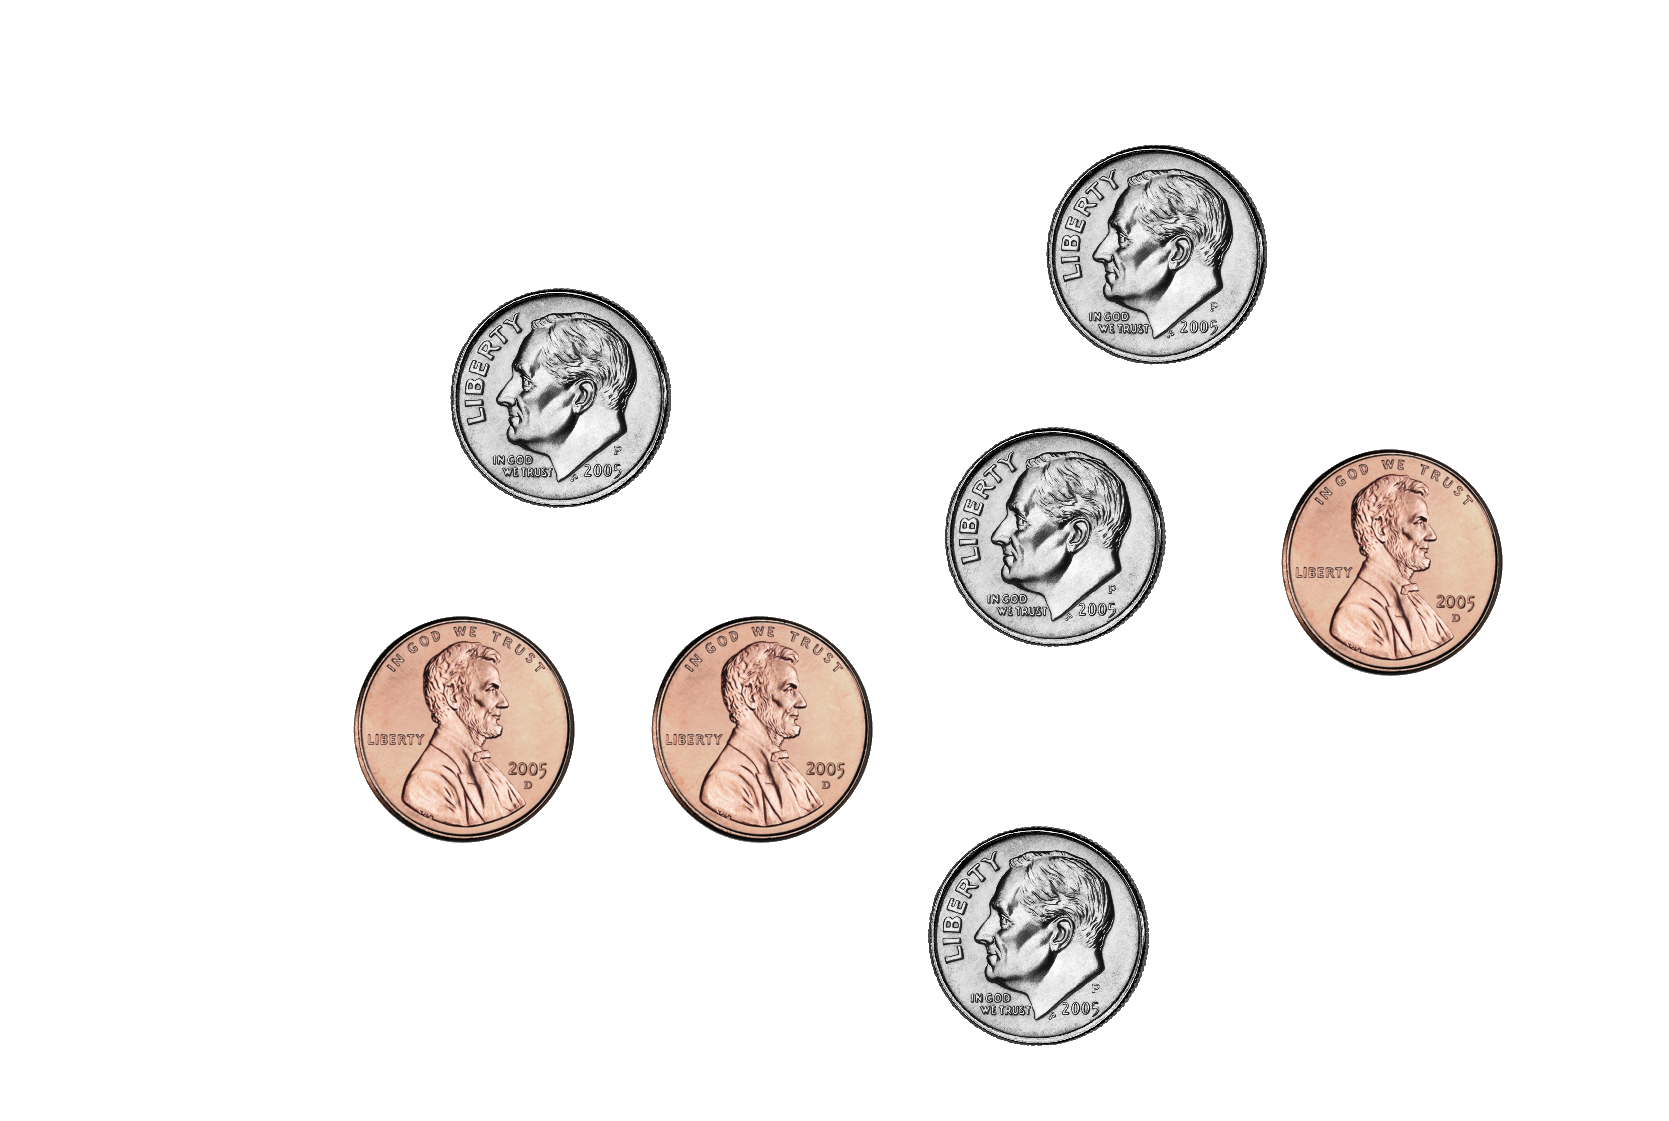
\includegraphics[height=1.7in]{takeawayCoins/07.pdf}
  }
\end{frame}

\begin{frame}
  Round 3a: Player $\pl A$ takes away 1 coin, leaving 6.

  \centerline{
    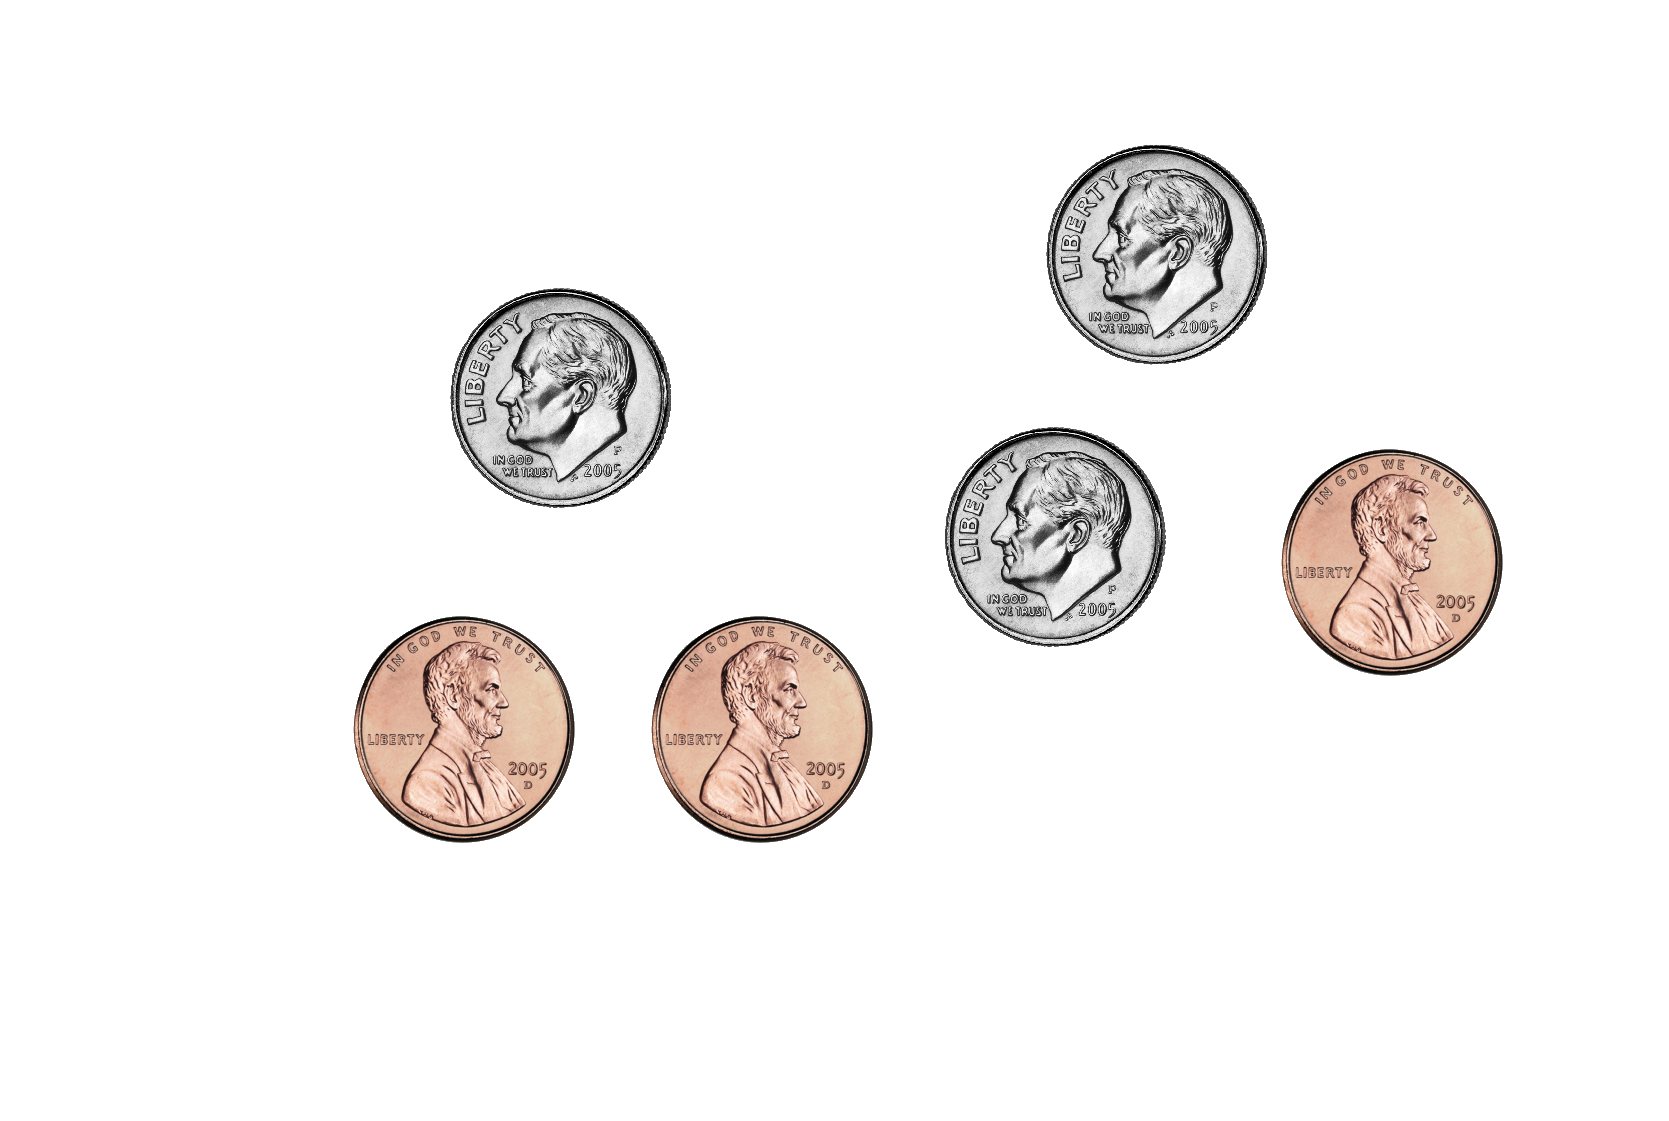
\includegraphics[height=1.7in]{takeawayCoins/06.pdf}
  }
\end{frame}

\begin{frame}
  Round 3b: Player $\pl B$ takes away 2 coins, leaving 4.

  \centerline{
    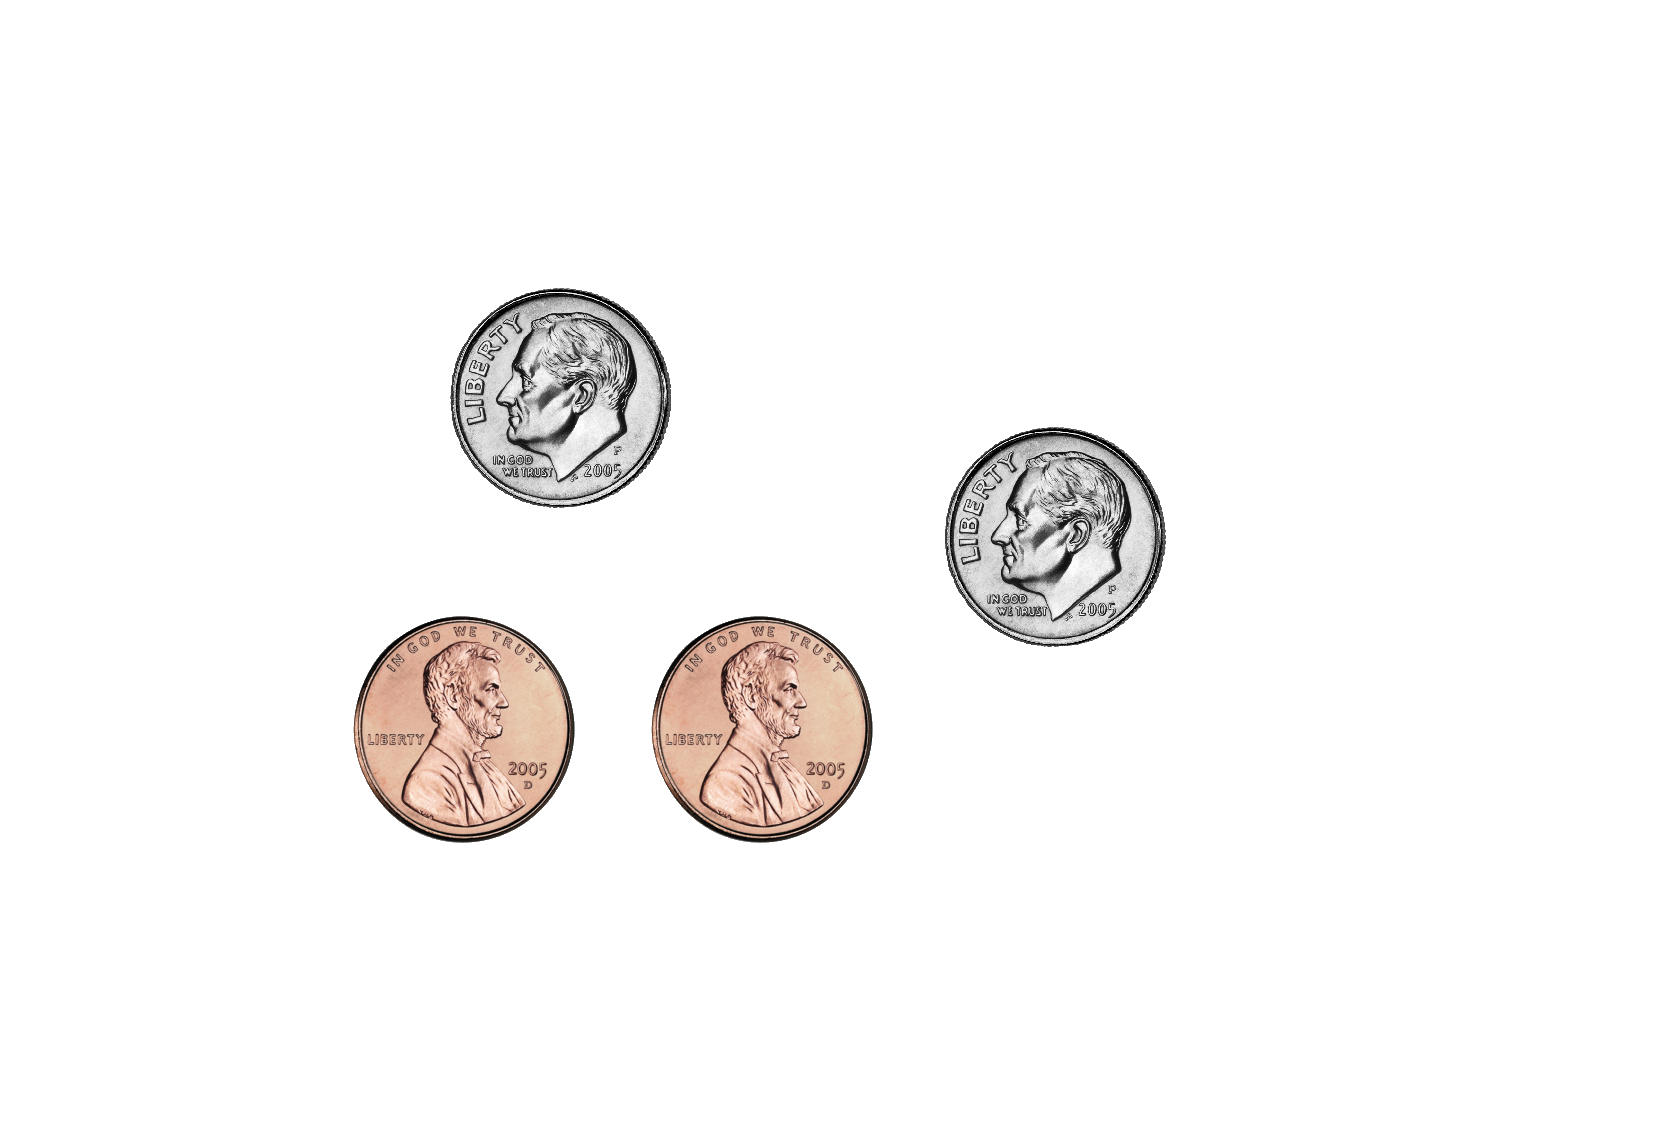
\includegraphics[height=1.7in]{takeawayCoins/04.pdf}
  }
\end{frame}

\begin{frame}
  Round 4a: Player $\pl A$ takes away 1 coin, leaving 3.

  \centerline{
    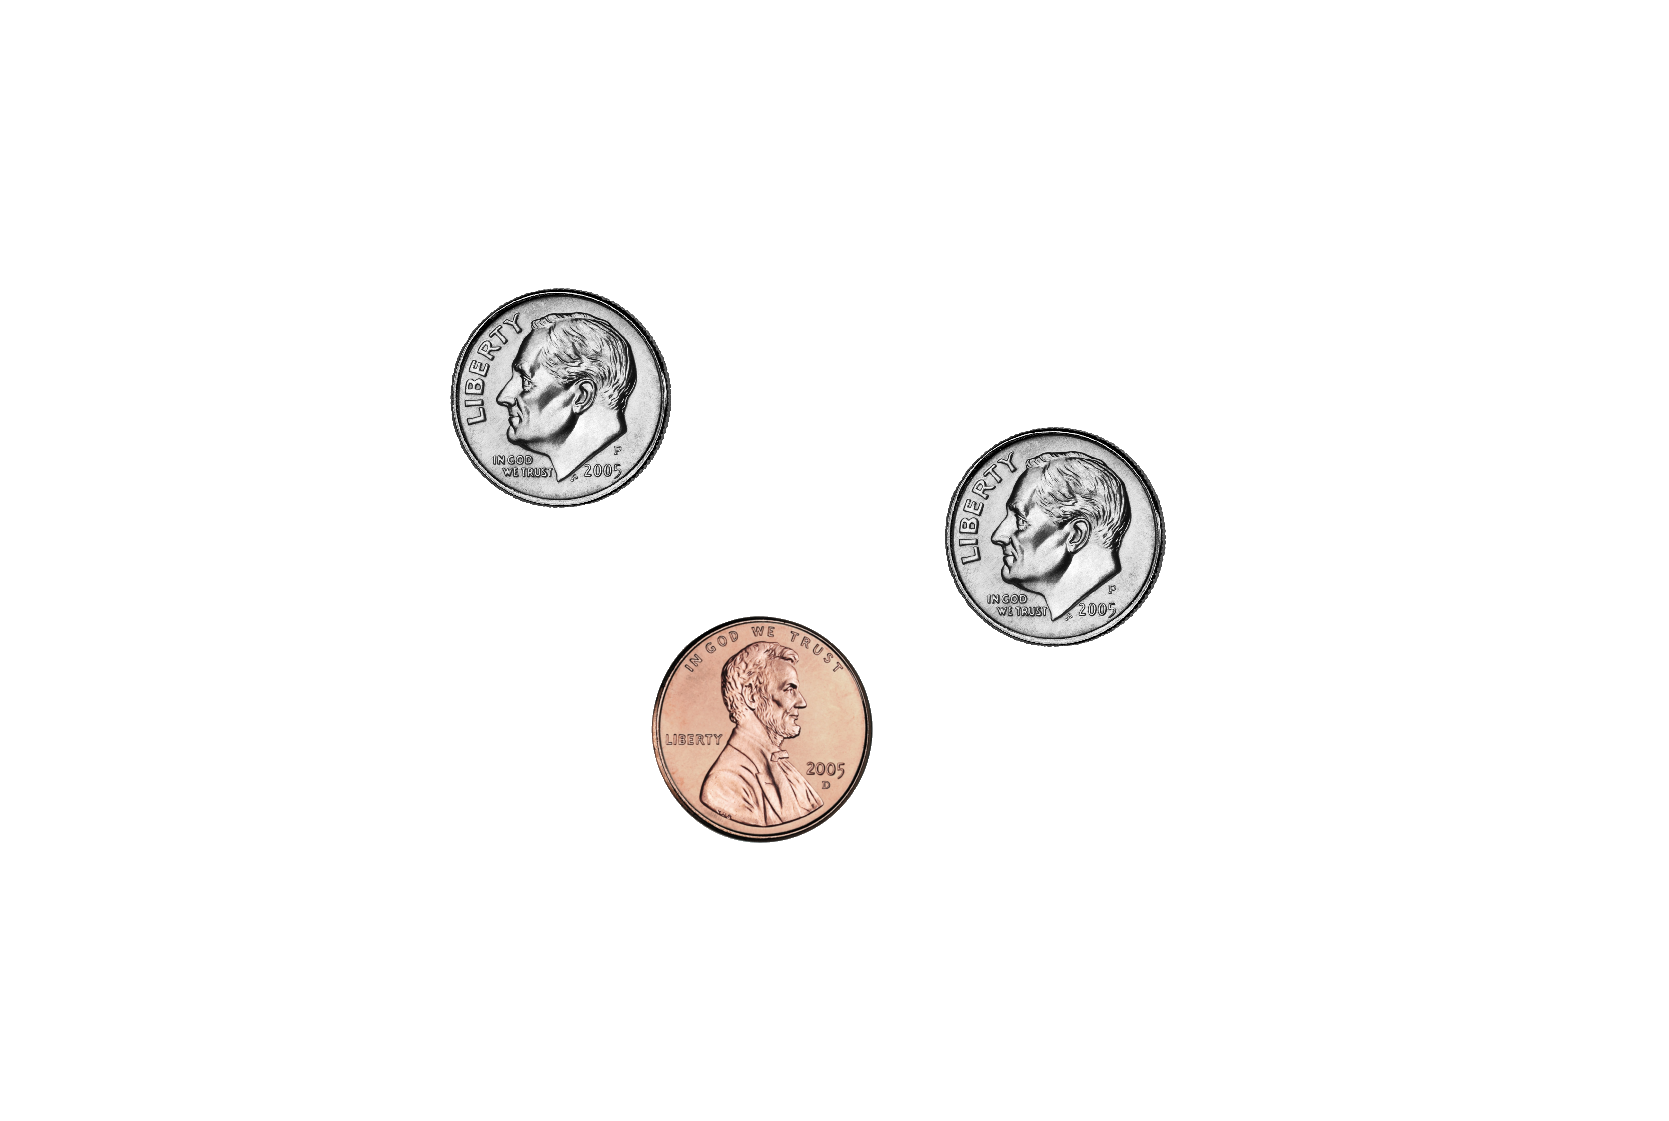
\includegraphics[height=1.7in]{takeawayCoins/03.pdf}
  }
\end{frame}

\begin{frame}
  Round 4b: Player $\pl B$ takes away the last 3 coins, and wins!

  \centerline{
    
\includegraphics[height=1.7in]{takeawayCoins/00.pdf}
  }
\end{frame}

\begin{frame}{A winning strategy}
  When studying sequential games, we often want to find what's called
  a \term{winning strategy}. Such a strategy should guarantee that the player
  following it cannot lose the game.

  \vpause

  I claim that when Takeaway starts with $12$ coins, then Player $\pl B$ has
  a winning strategy.

  \centerline{
    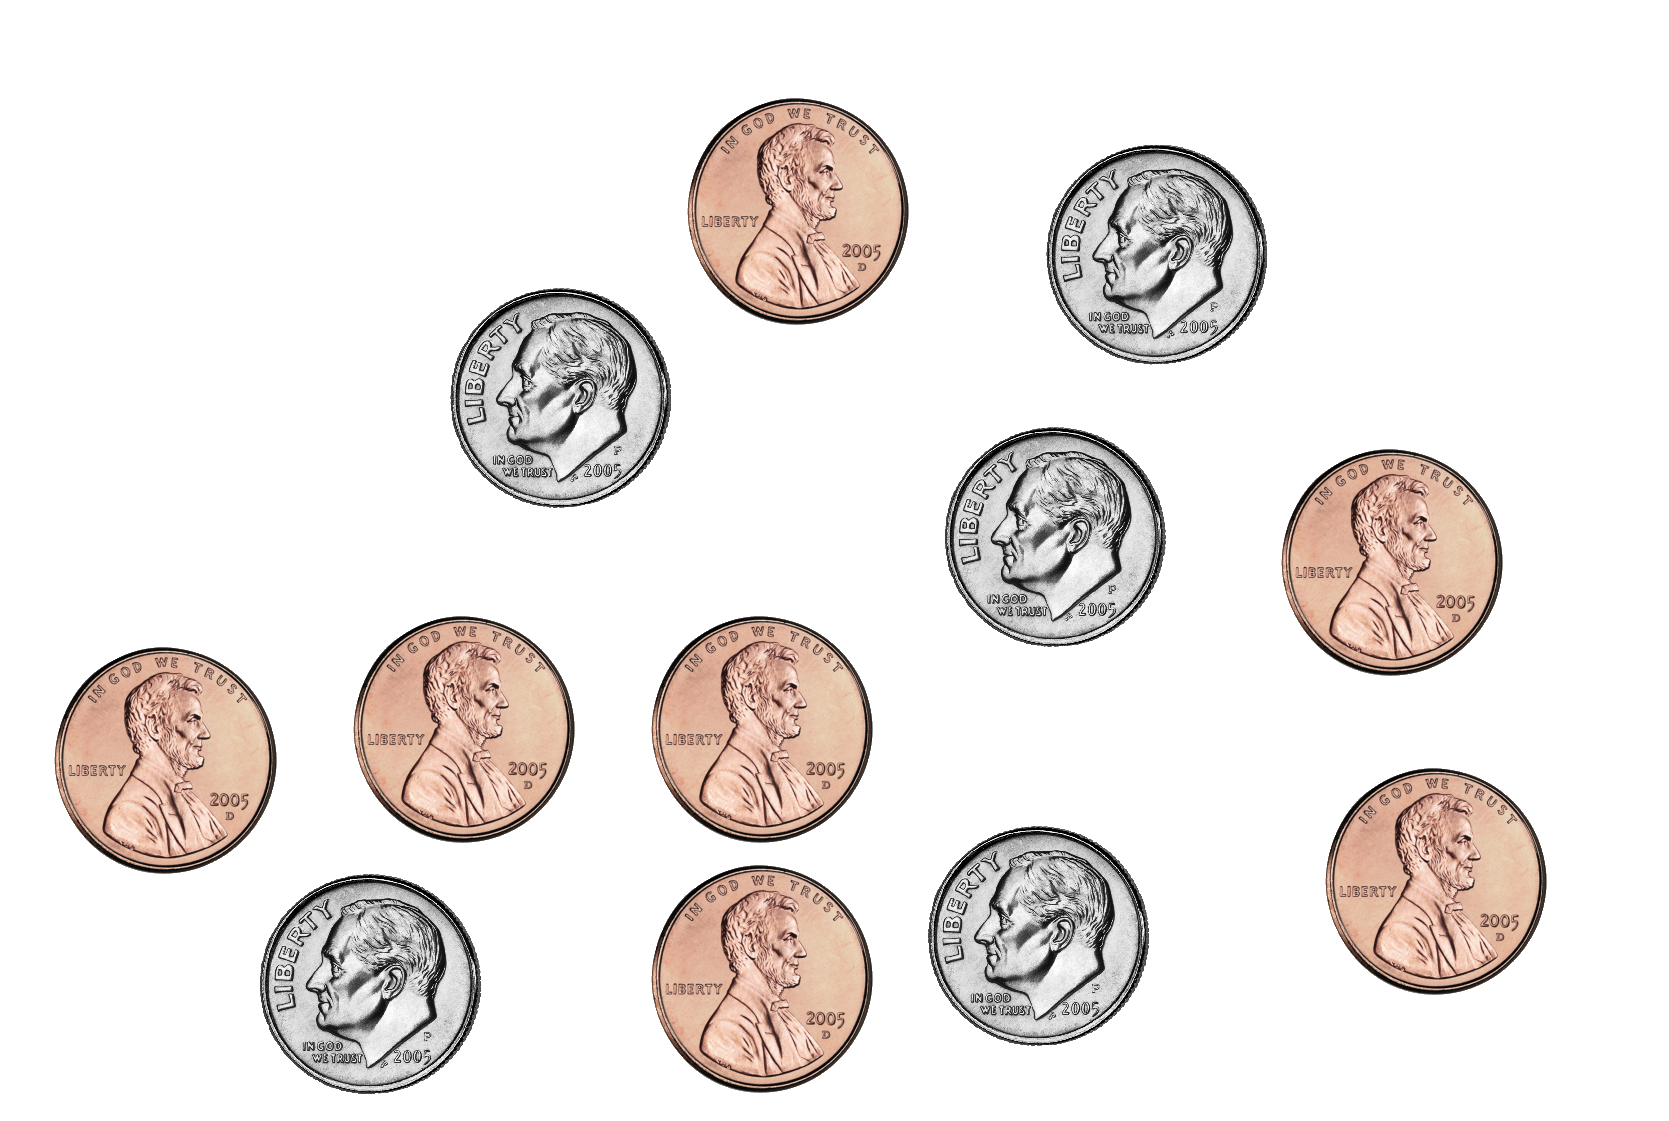
\includegraphics[height=1in]{takeawayCoins/12.pdf}
  }
\end{frame}

\begin{frame}
  \textbf{Proof:} Player $\pl B$ can always end her round so that there's $8$,
  then $4$, then $0$ coins. For example:

  \vpause

  {\small \begin{center}\begin{tabular}{cc}
    $12-1=11$ & $11-3=8$ \\
    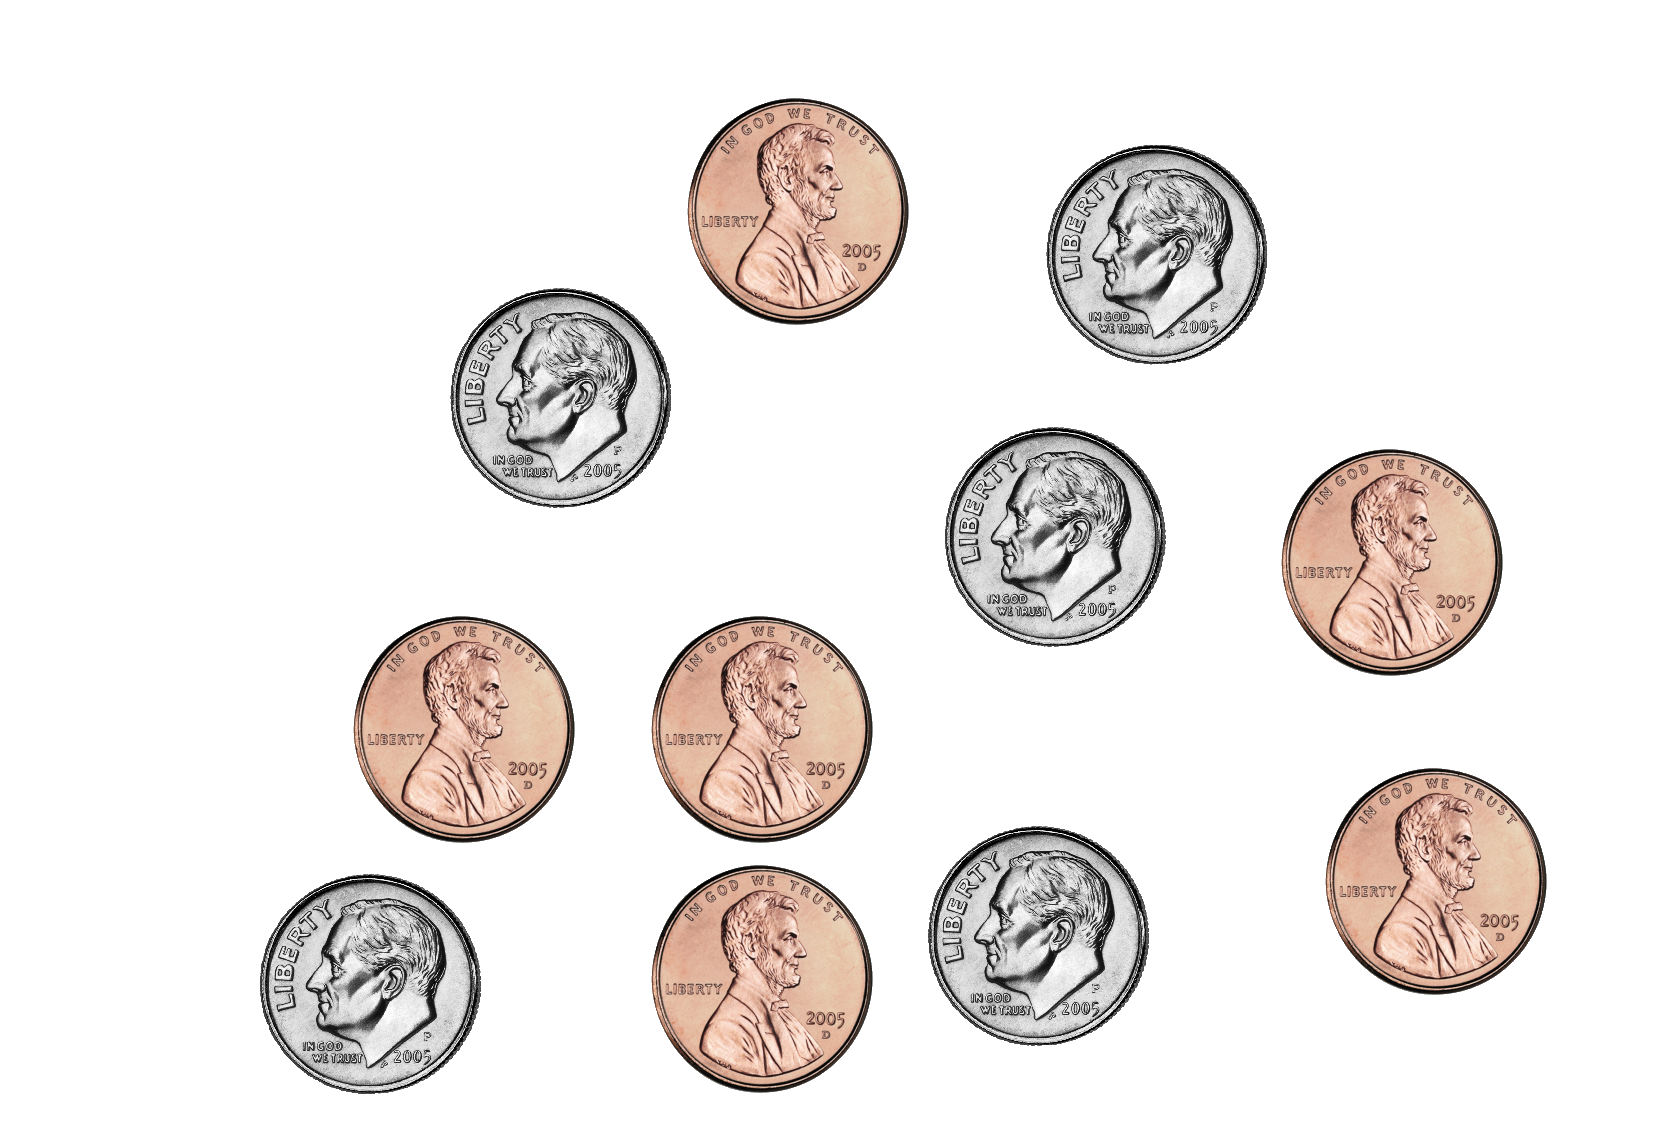
\includegraphics[height=0.5in]{takeawayCoins/11.pdf} &
    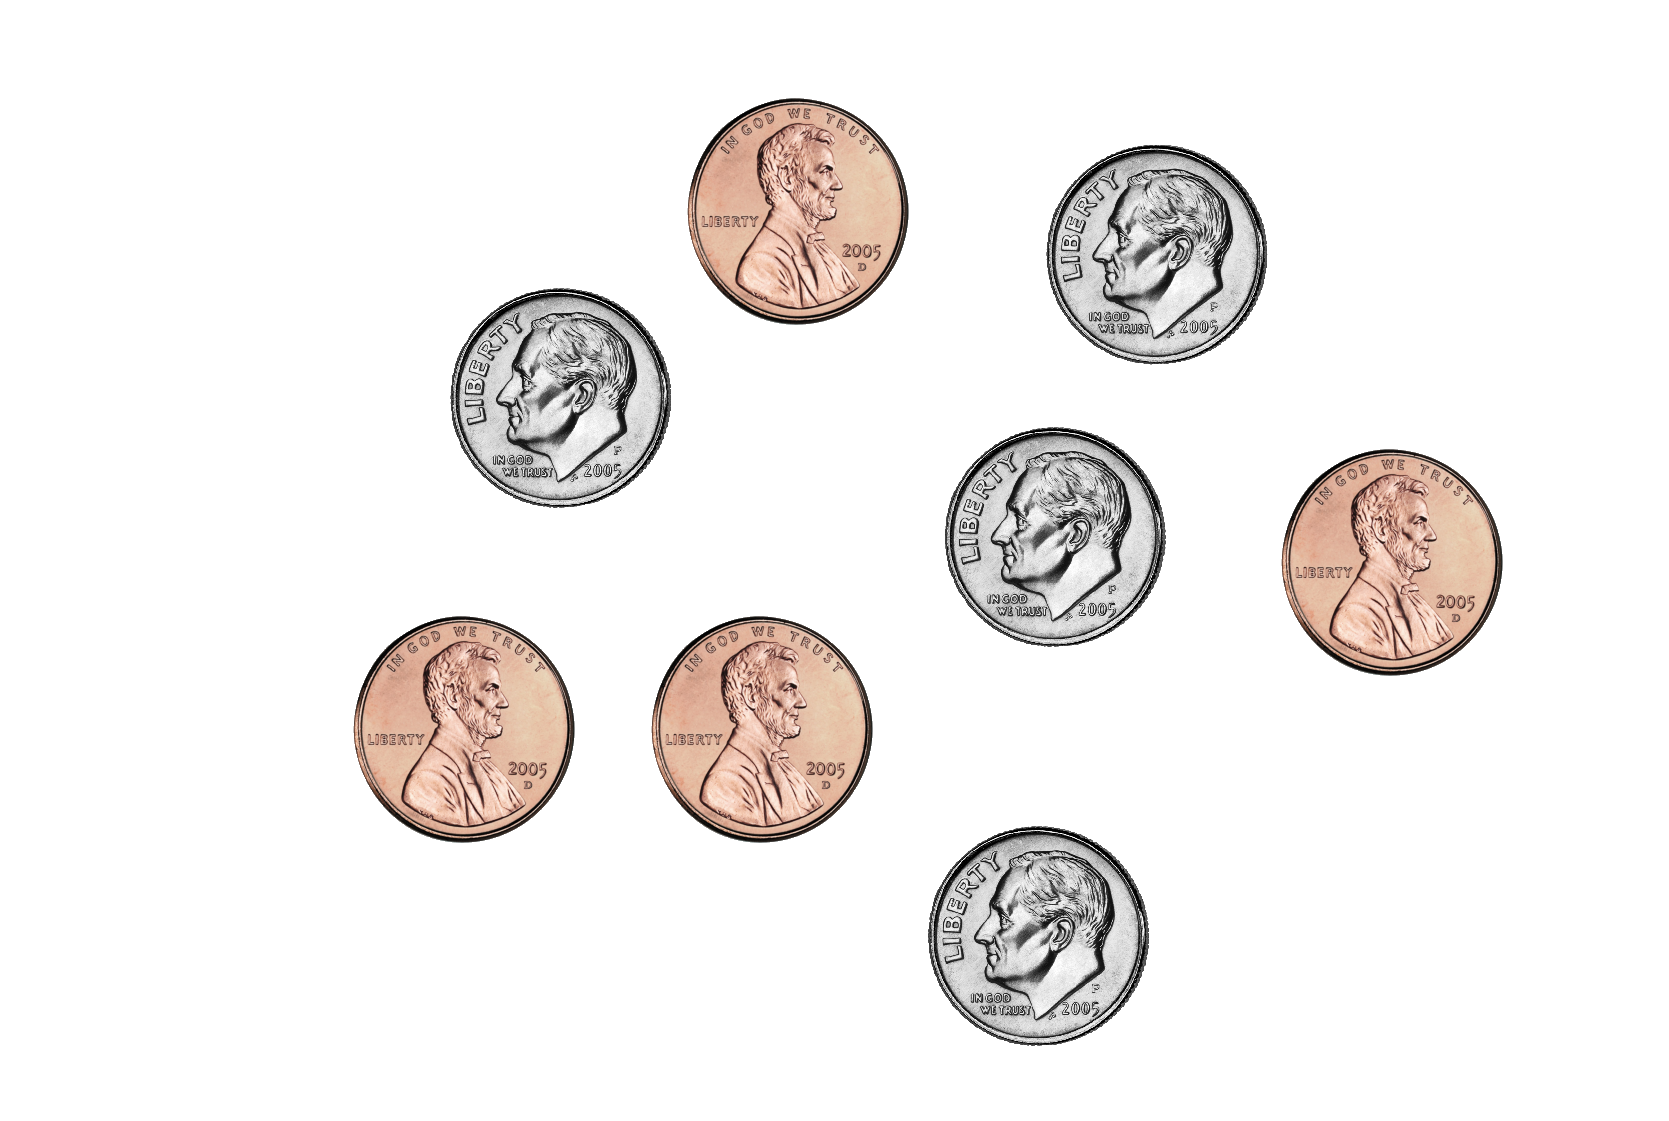
\includegraphics[height=0.5in]{takeawayCoins/08.pdf} \vspace{1em}\\

    $12-2=10$ & $10-2=8$ \\
    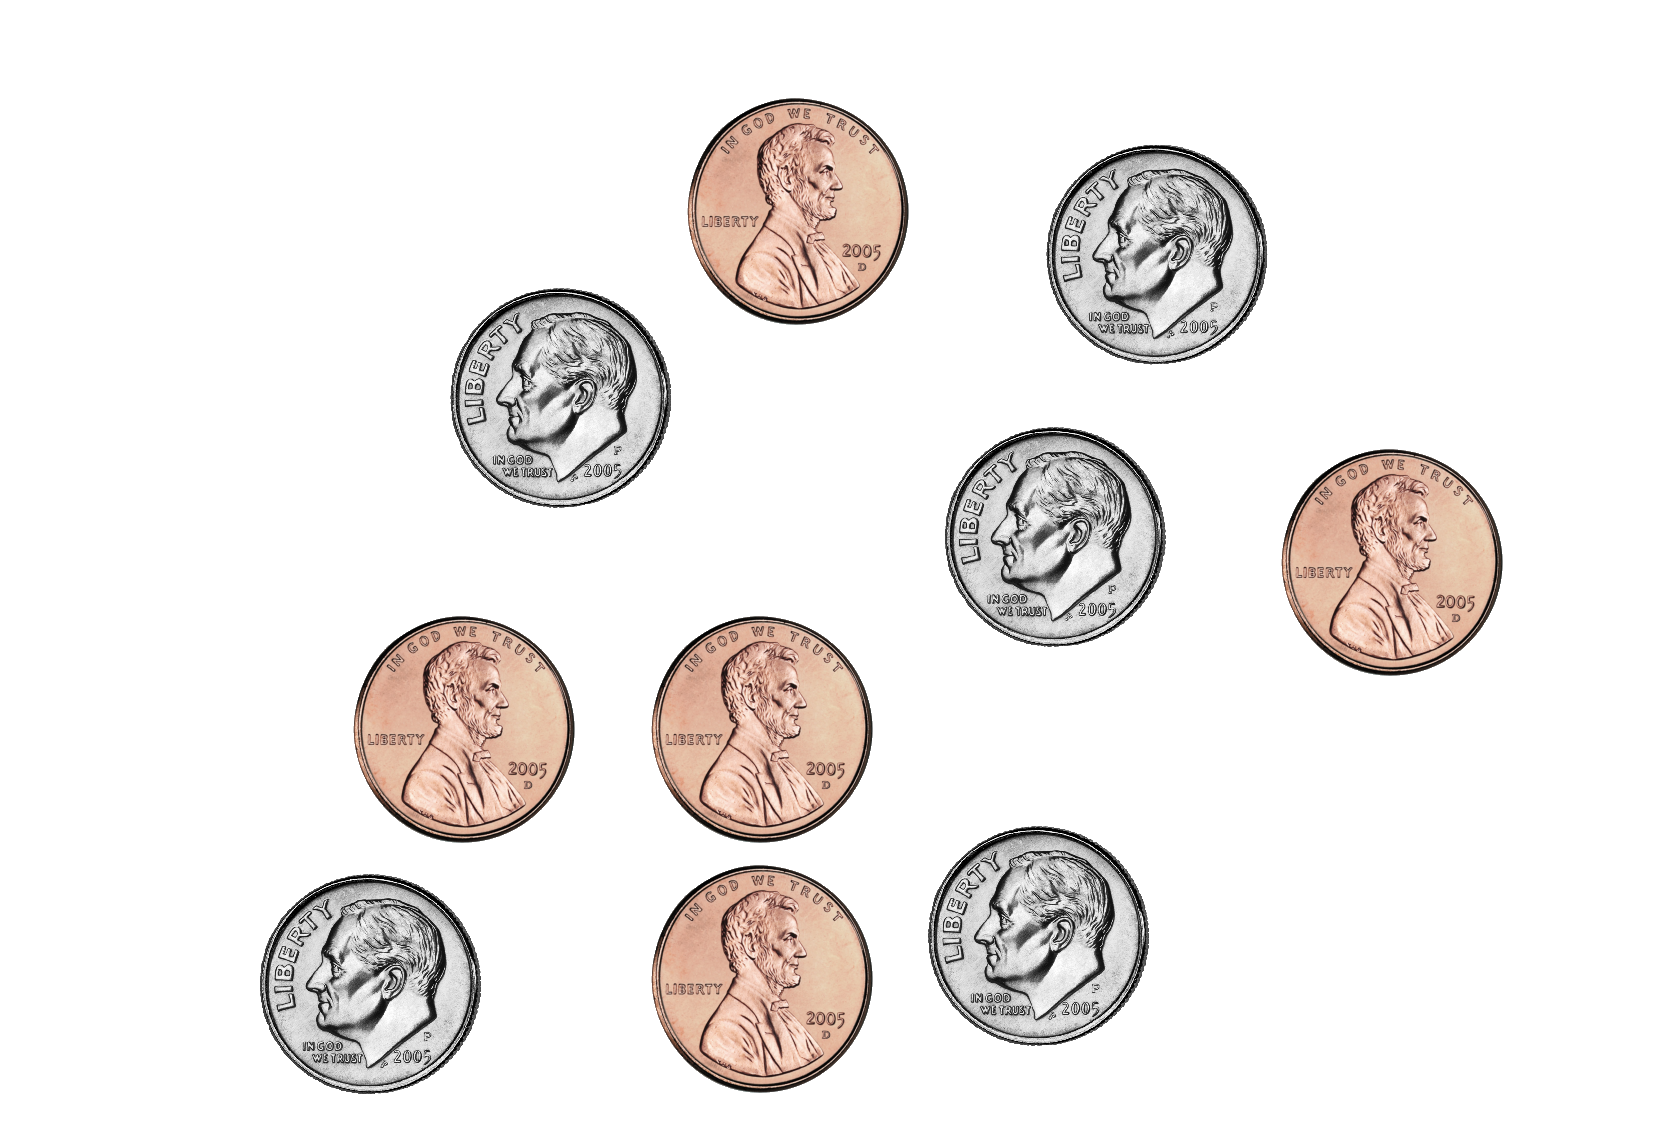
\includegraphics[height=0.5in]{takeawayCoins/10.pdf} &
    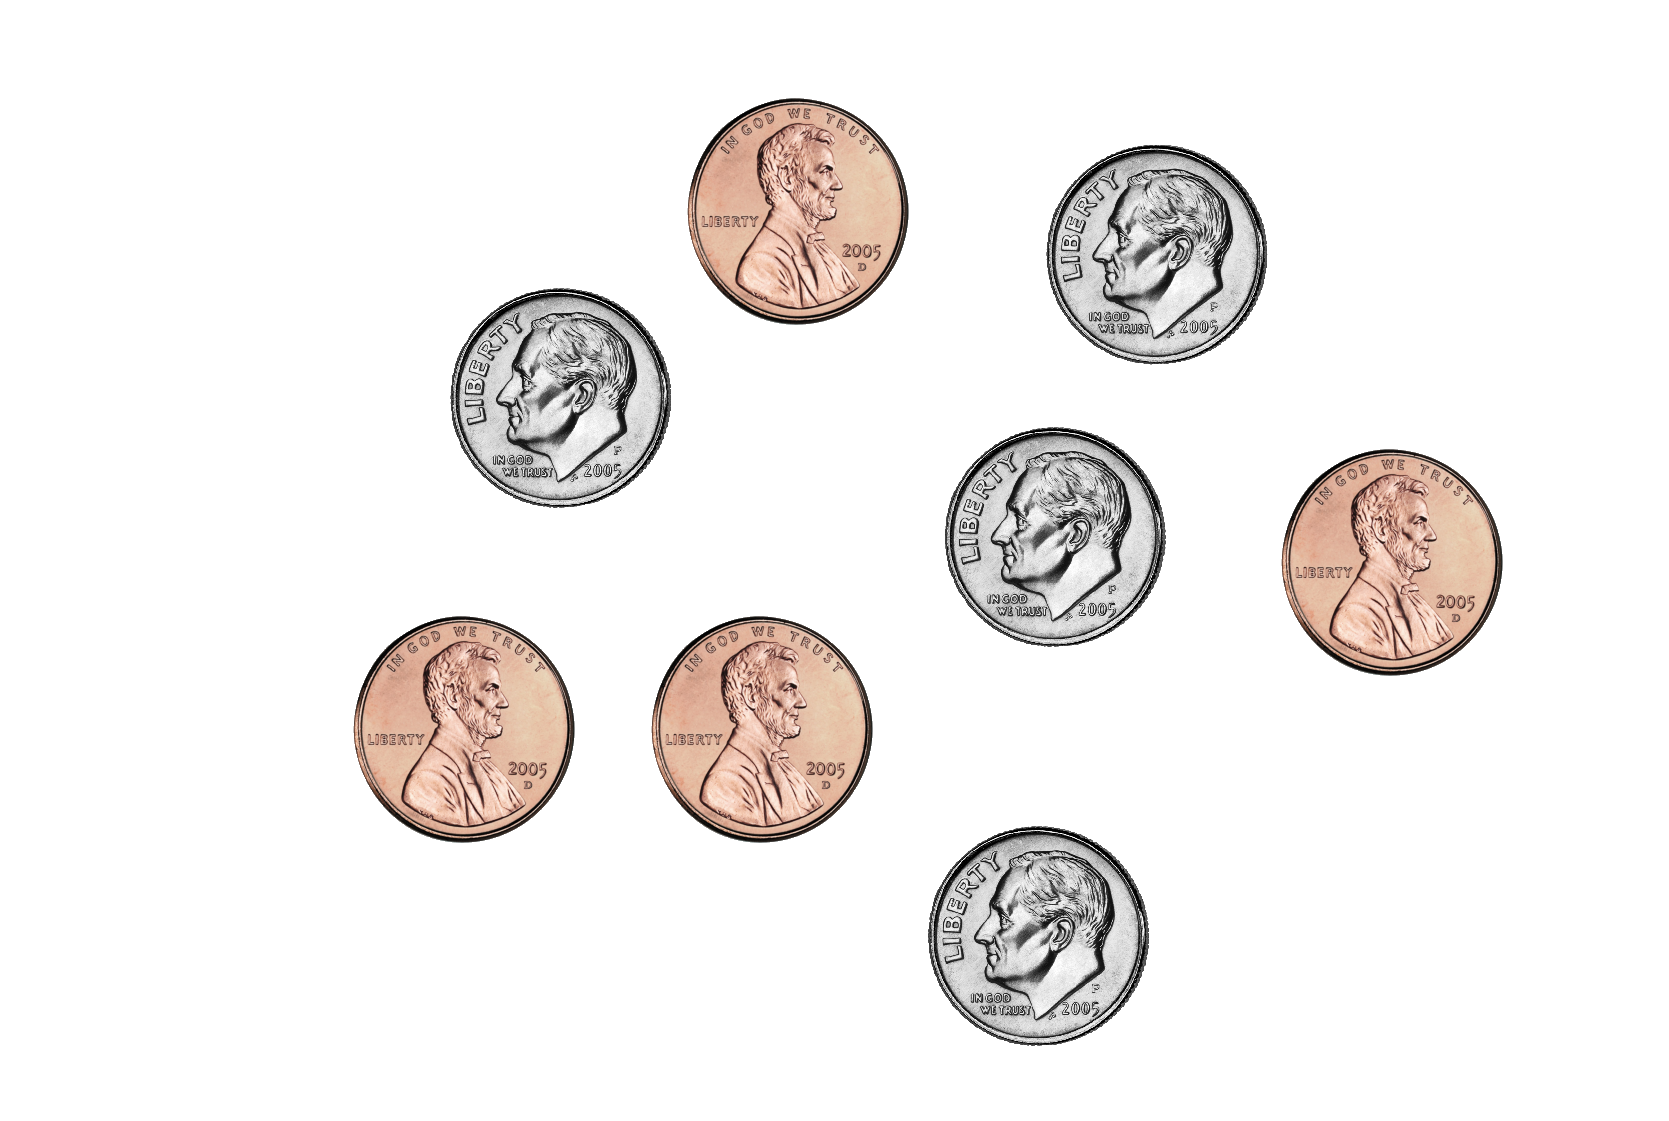
\includegraphics[height=0.5in]{takeawayCoins/08.pdf} \vspace{1em}\\

    $12-3=9$ & $9-1=8$ \\
    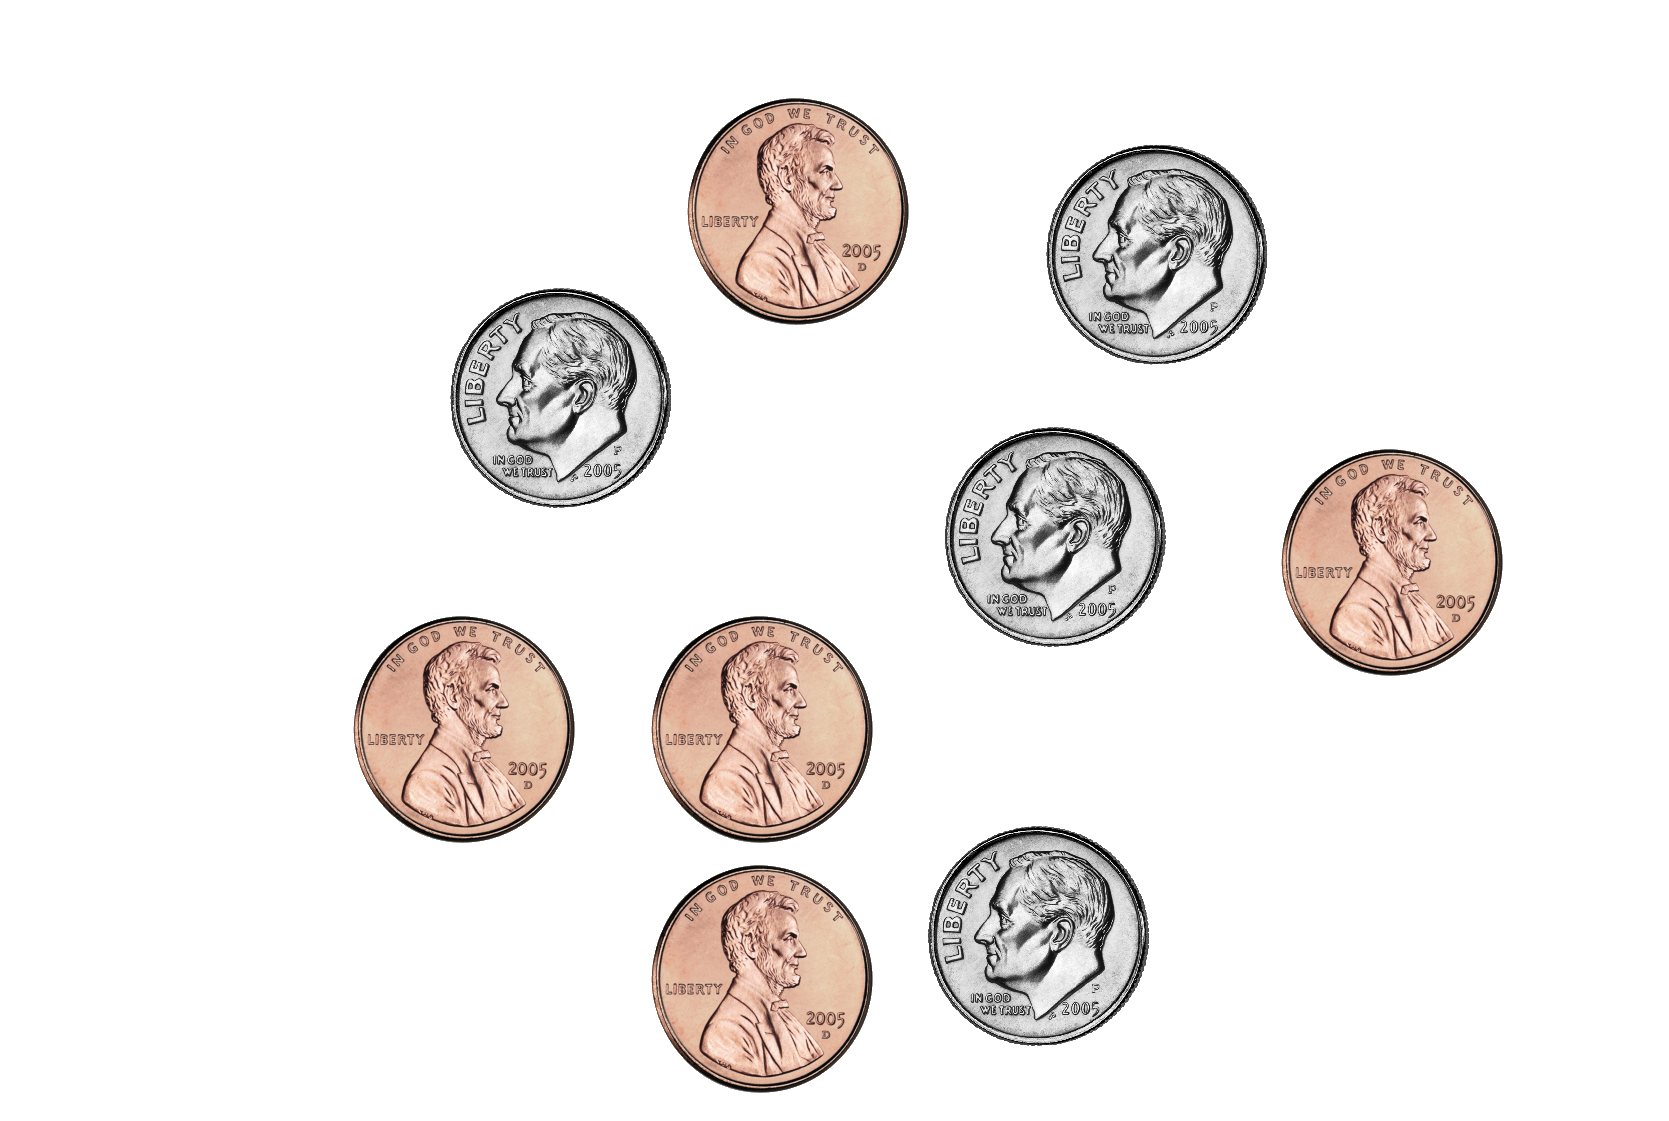
\includegraphics[height=0.5in]{takeawayCoins/09.pdf} &
    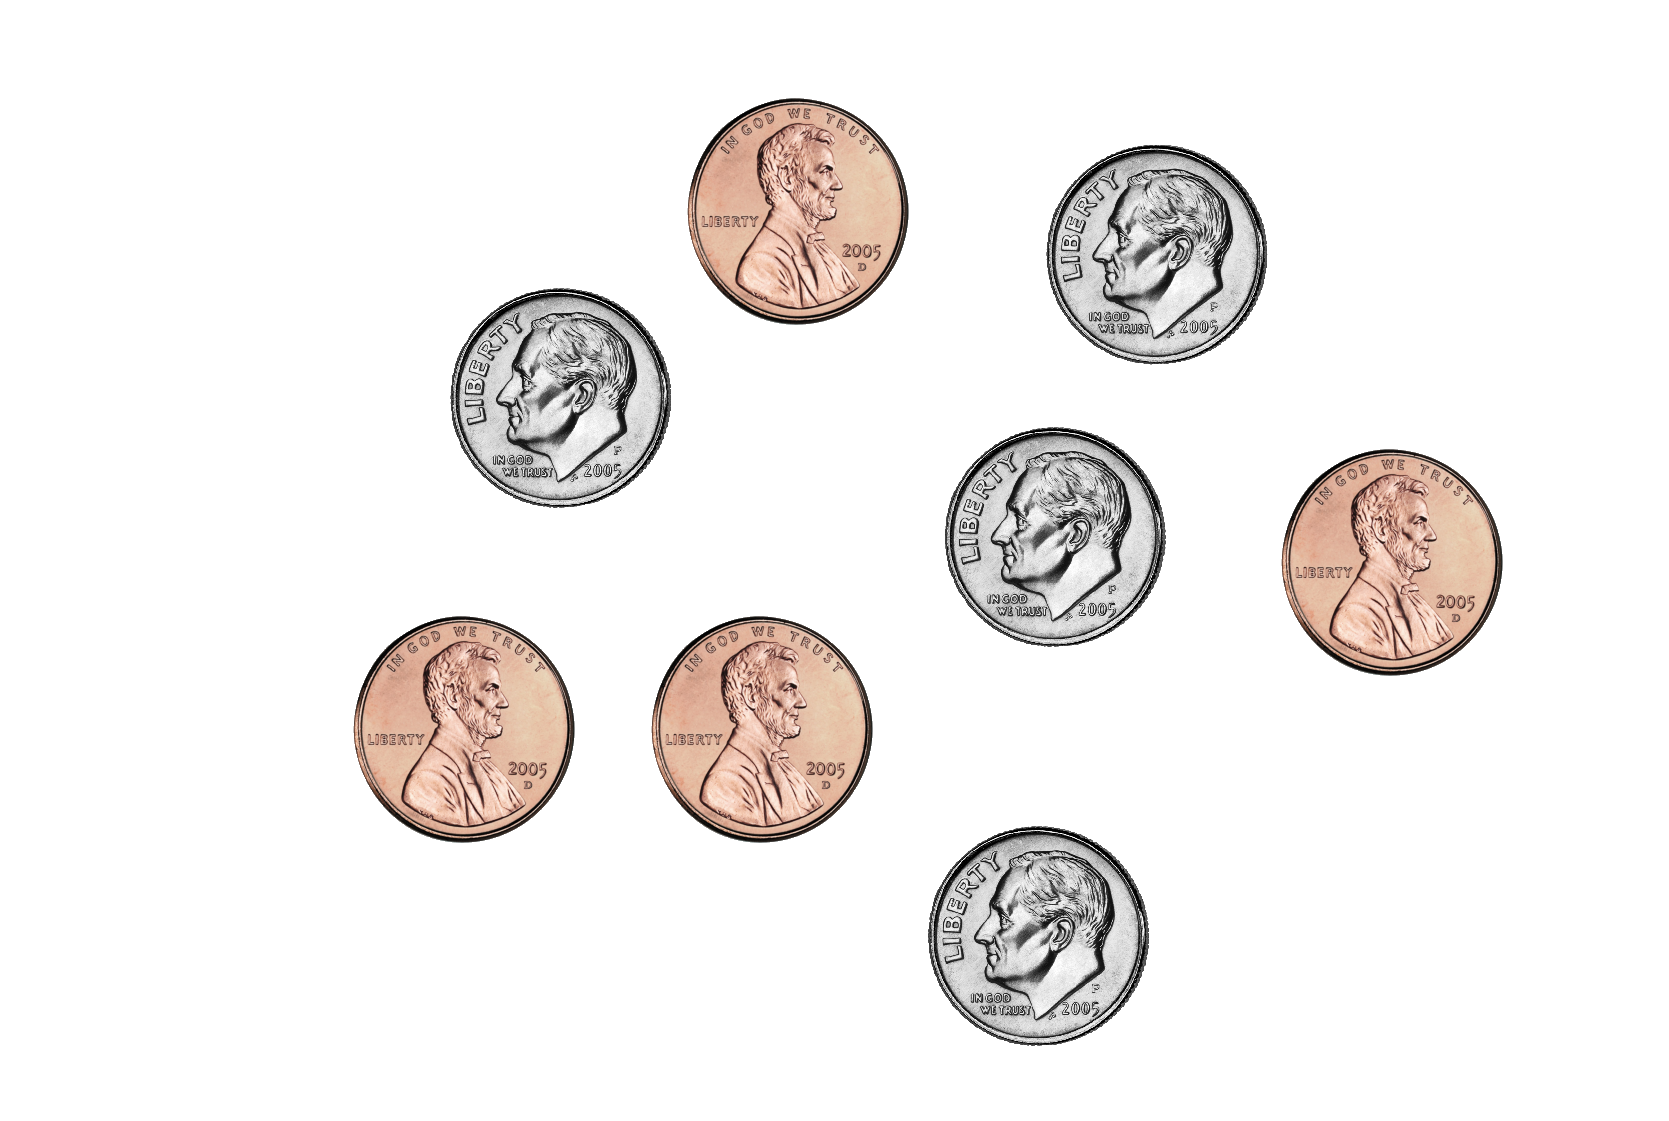
\includegraphics[height=0.5in]{takeawayCoins/08.pdf} \\
  \end{tabular}\end{center} }

\end{frame}

\begin{frame}
  Two puzzles to try out.

  \vpause

  \textbf{Puzzle 1:} Show that Player $\pl A$ had a winning strategy
  in Takeaway played with $15$ coins (which she obviously didn't follow
  in the example).

  \vpause

  \textbf{Puzzle 2:} Make a general rule about the number of starting coins
  which tells whether Player $\pl A$ or $\pl B$ has a winning strategy.
\end{frame}


% \subsection{Anatomy of a Game}

% \begin{frame}{Heads up}
%   This talk is about \term{sequential} or \term{combinatorial} games
%   of perfect information.

%   \vpause

%   Game theory is a broad subject, including classic games like the
%   \term{Prisoner's Delimma} where two players make a \term{simultaneous}
%   choice, or \term{Yahtzee} where the players face randomness from
%   dice rolls.

%   \vpause

%   However, we're going to look at games in the family of \term{Tic Tac Toe}
%   or \term{Chess}, where two players take turns making moves with full knowledge
%   of their options and the history of their previous moves.
% \end{frame}

% \begin{frame}{Some Definitions}
%   \begin{definition}
%     Let $\omega=\{0,1,2,\dots\}$, and let $B^A$ be the set of all functions
%     with domain $A$ and range $B$.

%     Then $X^\omega$ contains all functions from $\{0,1,2,\dots\}$ to $X$, or
%     equivalently, all sequences of the form $\<x_0,x_1,x_2,\dots\>$ with
%     $x_i\in X$.
%   \end{definition}
%   \pause
%   \begin{definition}
%     A \term{game} $G$ is a tuple $\<M,W\>$ where $W\subseteq M^\omega$.
%     $M$ represents the set of possible moves of the game, and $W$ contains
%     certain sequences of moves $\<a_0,b_0,a_1,b_1,\dots\>$ called
%     \term{victories} (for the first player).
%   \end{definition}
% \end{frame}

% \begin{frame}
%   In this context, all games have two players, and there are no ties.

%   \vpause

%   If the players of the game are $\pl A$ and $\pl B$, then a \term{playthrough}
%   of the game is some sequence in $M^\omega$:
%   \[
%     p=\<a_0,b_0,a_1,b_1,a_2,b_2,\dots\>
%   \]

%   \pause

%   If $p$ is in $W$, then the first player $\pl A$ has won the game; otherwise,
%   the second player $\pl B$ has won the game.
% \end{frame}

% \begin{frame}{Example}
%   As an example, let $\<M,W\>$ be the game \term{Sylver Coinage} with players
%   $\pl A$, $\pl B$ where $M=\{2,3,4,\dots\}$.

%   \vpause

%   Defining $W$ directly as a set is usually obnoxious, so we'll define it
%   implicitly by setting this rule: no player can choose a number which is
%   the sum of previously chosen numbers, perhaps with repetition.

%   \vpause

%   Thus, if $4$ and $7$ have been chosen previously, then $25=4+7+7+7$ is not a
%   legal move.

%   \vpause

%   Thus a sequence $\<a_0,b_0,a_1,b_1,\dots\>$ will be in $W$ if it shows the
%   second player $\pl B$ breaking the rules before the first player $\pl A$.
% \end{frame}

% \begin{frame}
%   For example, consider the playthrough beginning with
%   \[
%     \<4,11,6,5,7,3,2,\dots\>
%   \]
%   \begin{itemize}
%     \item $\pl A$ chose $4$
%     \item $\pl B$ chose $11$
%     \item $\pl A$ chose $6$ (legal moves remaining:
%           $\{2,3,5,7,9,13\}$)
%     \item $\pl B$ chose $5$ (legal moves remaining:
%           $\{2,3,7\}$)
%     \item $\pl A$ chose $7$ (legal moves remaining:
%           $\{2,3\}$)
%     \item $\pl B$ chose $3$ (legal moves remaining: $\{2\}$)
%     \item $\pl A$ chose $2$ (legal moves remaining: $\emptyset$)
%     \item $\pl B$ chose something illegal and lost.
%   \end{itemize}
% \end{frame}

% \begin{frame}
%   This game, invented by John Conway, is an example of a \term{finite game},
%   since eventually one of the players are forced to break the given rules.
%   (A puzzle I'll leave for you to work on!)

%   \vpause

%   We've just seen that every sequence of the form $\<4,11,6,5,7,3,2,\dots\>$
%   is in $W$, since $\pl A$ wins those playthroughs of the game.
%   (Actually, another puzzle: show that all sequences of the form
%   $\<4,11,6,5,7,\dots\>$ are in $W$.)

%   \vpause

%   An artifact of this game model is that all playthroughs are infinite
%   sequences. After $\pl B$ makes an illegal move, there's no point to keep
%   playing in reality, but the sequences in $W$ stretch on in every possible
%   combination...
% \end{frame}

% \subsection{Strategies and Determinacy}

% \begin{frame}{Strategies}
%   \begin{definition}
%     A \term{strategy} is a function $\sigma$ which turns a finite sequence
%     of moves in $M$ into a new move in $M$.
%   \end{definition}

%   \pause

%   Put another way, a strategy is a fixed rule which tells a player what move
%   to make during each round \textit{in response} to all the previous moves
%   of the game.
% \end{frame}

% \begin{frame}{Attacks}
%   \begin{definition}
%     An \term{attack} is sequence of moves in $M$.
%   \end{definition}

%   \pause

%   Put another way, an attack is a fixed rule which tells a player what move
%   to make during each round \textit{ignoring} all the previous moves of
%   the game.
% \end{frame}

% \begin{frame}{Winning Strategies}
%   \begin{definition}
%     The \term{result} of a game for which $\pl A$ uses the strategy $\sigma$
%     $\pl B$ uses the attack $\<b_0,b_1,\dots\>$ is the playthrough of the
%     game $\<\sigma(\emptyset),b_0,\sigma(b_0),b_1,\sigma(b_0,b_1),\dots\>$
%   \end{definition}

%   (Or the similar definition when $\pl B$ has a strategy and $\pl A$
%   has an attack.)

%   \pause

%   \begin{definition}
%     If $\sigma$ is a strategy for $\pl A$ such that the result of the game for
%     every possible attack by $\pl B$ is in $W$, then $\sigma$ is a
%     \term{winning strategy}.
%   \end{definition}

%   (Or the similar definition when $\pl B$ has a strategy, and all results
%   are not in $W$.)
% \end{frame}

% \begin{frame}
%   \begin{definition}
%     If one of the players has a winning strategy for a game, then that
%     game is said to be \term{determined}.
%   \end{definition}

%   Obviously, both players can't have a guaranteed way to win the same
%   game, but is it possible that neither player can guarantee a way to win?
%   That is, for every fixed strategy by either player, could the opponent
%   always have some chance of getting lucky and beating it?
% \end{frame}

% \section{Determinacy of Finite Games}

% \subsection{Borel Determinacy Theorem}

% \begin{frame}{Borel Determinacy Theorem}
%   We could use a very strong topological and set-theoretic result to prove
%   that finite games are determined.

%   \begin{theorem}
%     If $M$ is given the discrete topology, and $M^\omega$ is given the usual
%     product topology, then the game $G=\<M,W\>$ is determined whenever $W$
%     is a Borel subset of the space $M^\omega$.
%   \end{theorem}

%   \pause

%   With a little topology, you can show that if $G$ is finite, then $W$ is
%   an open set, which implies it's Borel. Thus finite games \textit{are}
%   determined: one of the players has a winning strategy.

%   \vpause

%   Of course, all that requires a few semesters of graduate topology to grok,
%   so maybe there's a better way...
% \end{frame}

% \subsection{Decision Tree Proof}

% \begin{frame}{Decision Trees}
%   Finite games can be modeled as a decision tree.

%   \centerline{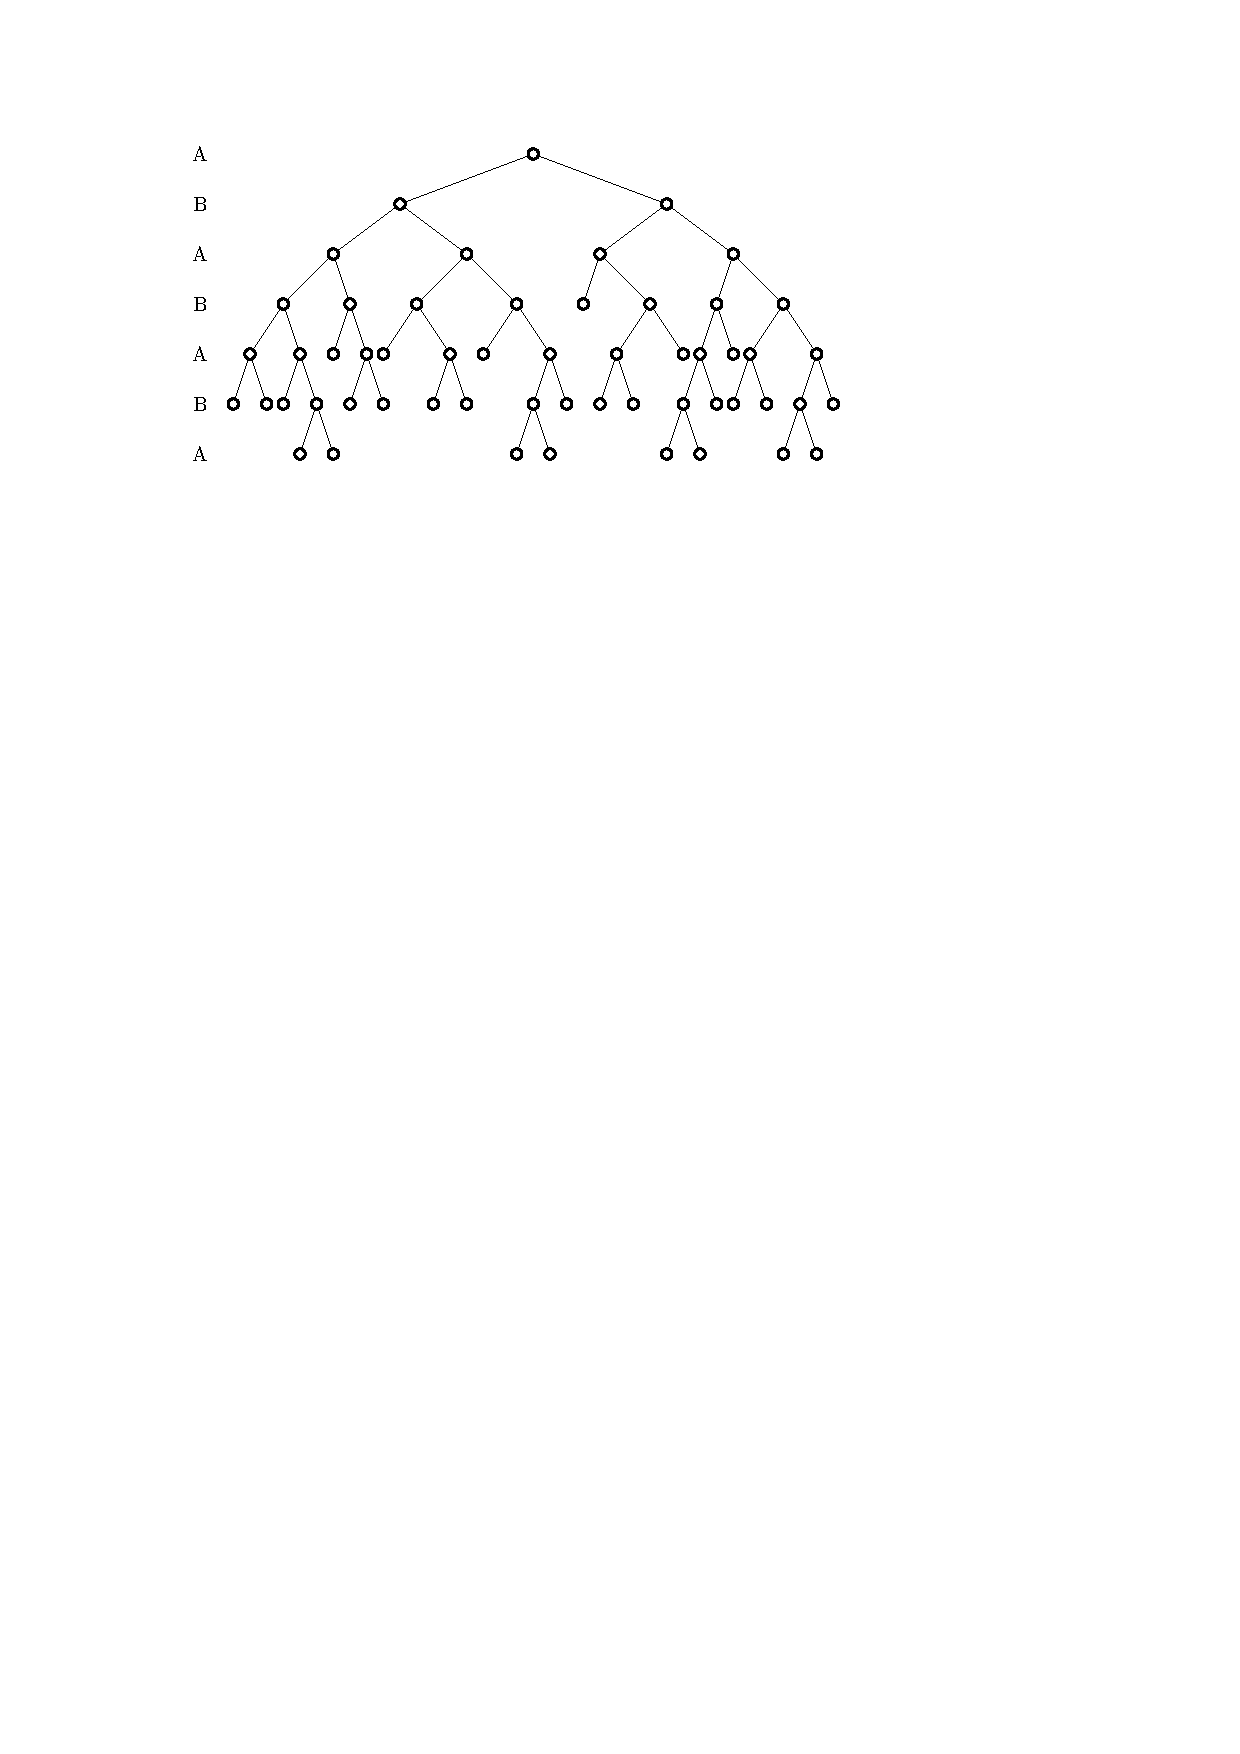
\includegraphics[width=3in]{decisionTree1.pdf}}

%   The above tree models a game where $\pl A$ and $\pl B$ alternate choosing
%   ``left'' or ``right'' moves to descend the tree. A player wins if they
%   move into a terminal node of the tree, since the opponent cannot move farther.
% \end{frame}

% \begin{frame}
%   \centerline{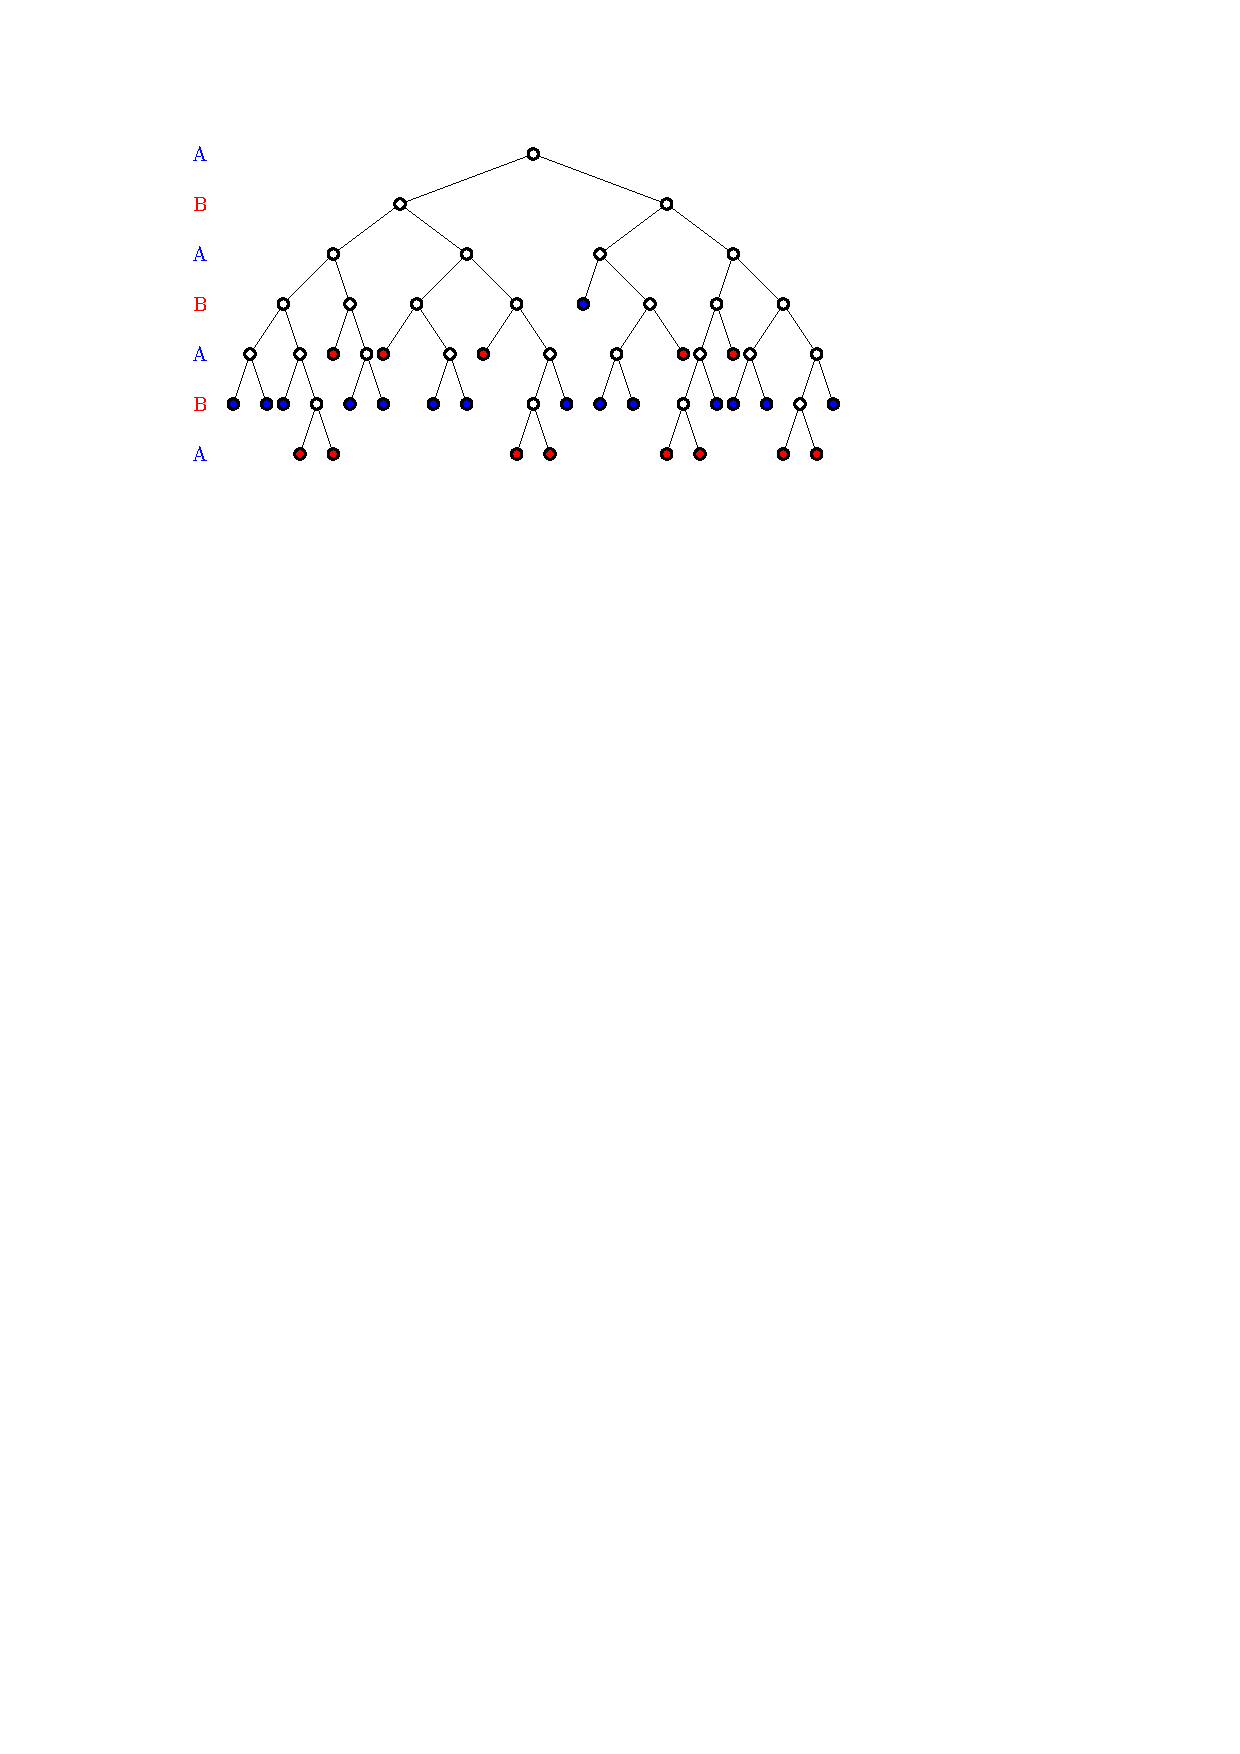
\includegraphics[width=3in]{decisionTree2.pdf}}

%   \vspace{1em}

%   We can label the tree by first showing the states where $\pl A$ (blue) and
%   $\pl B$ (red) have already won the game.
% \end{frame}

% \begin{frame}
%   \centerline{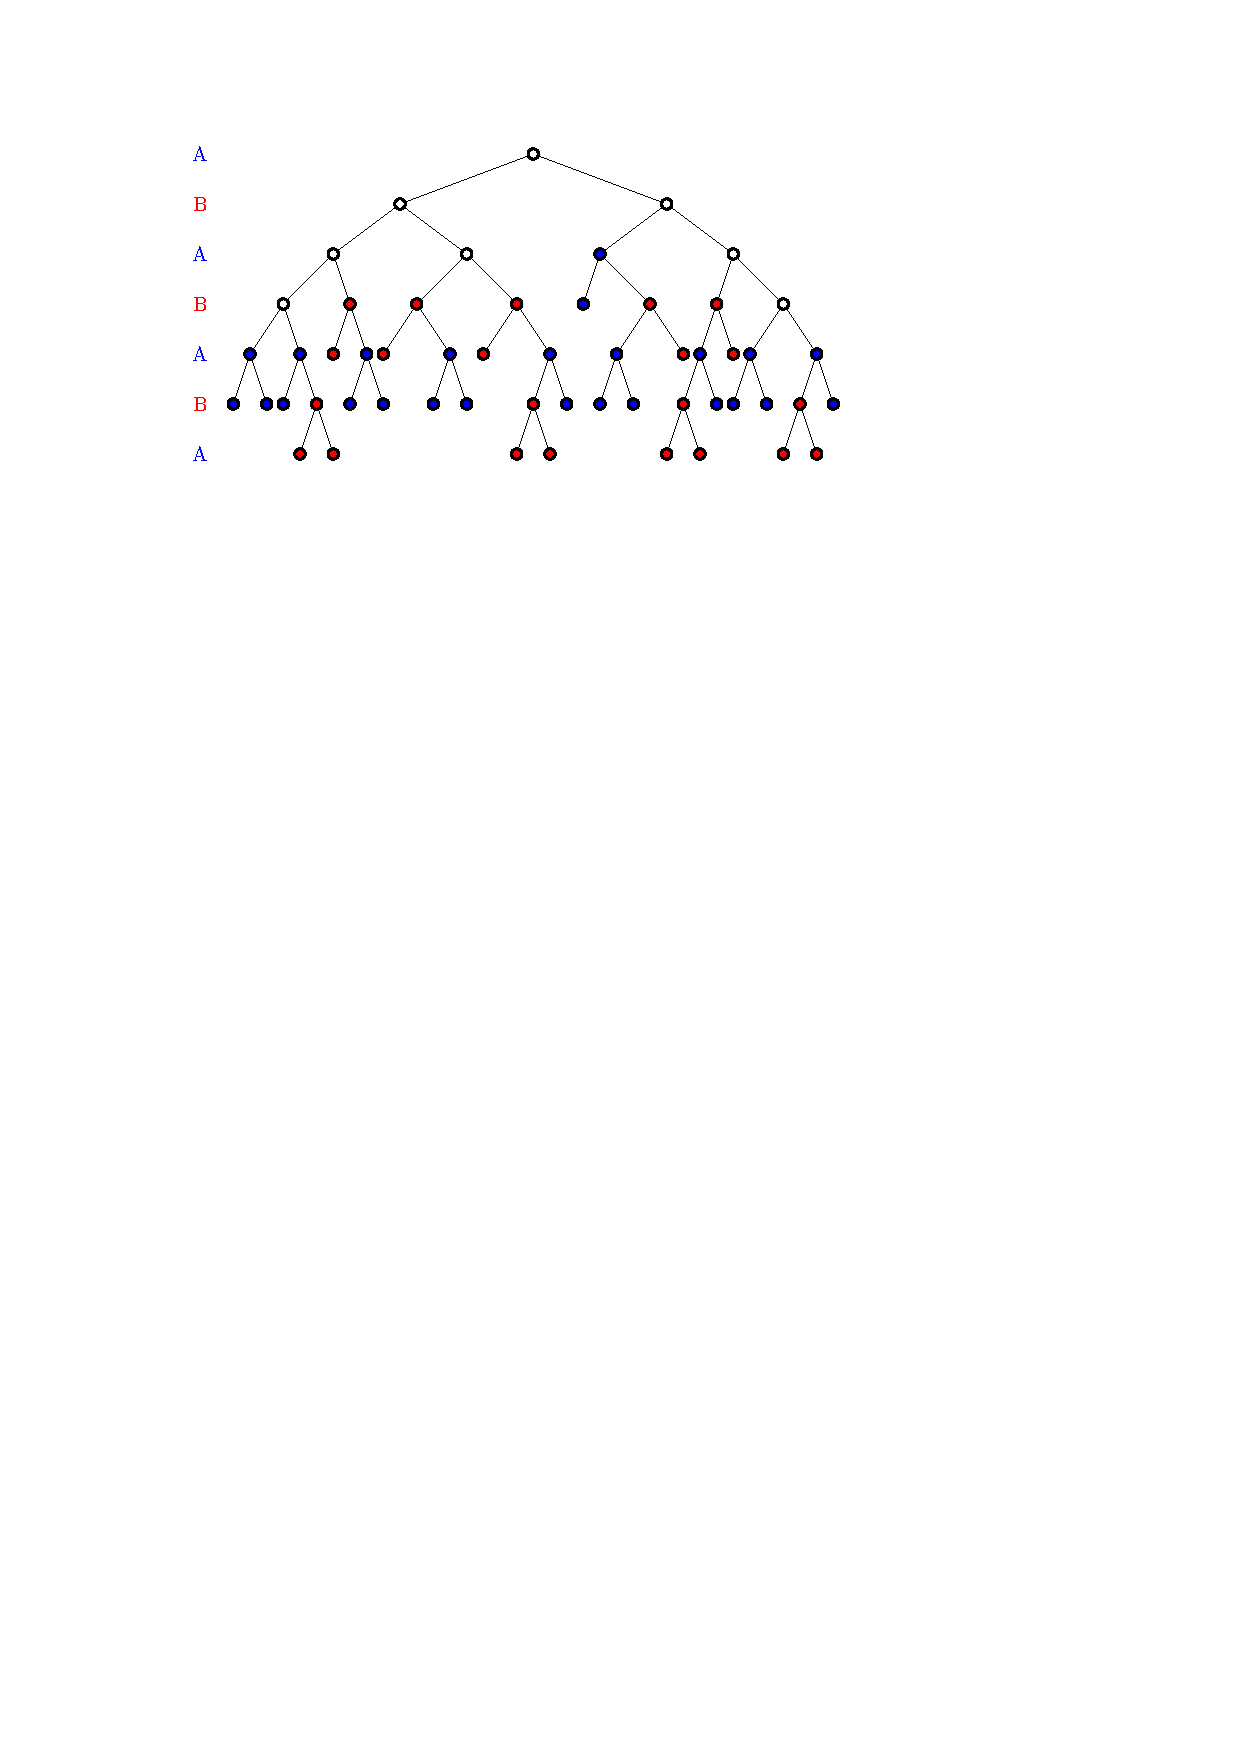
\includegraphics[width=3in]{decisionTree3.pdf}}

%   \vspace{1em}

%   Then, we can move back and label the spaces where the active player is able
%   to move to a vertex of their color.
% \end{frame}

% \begin{frame}
%   \centerline{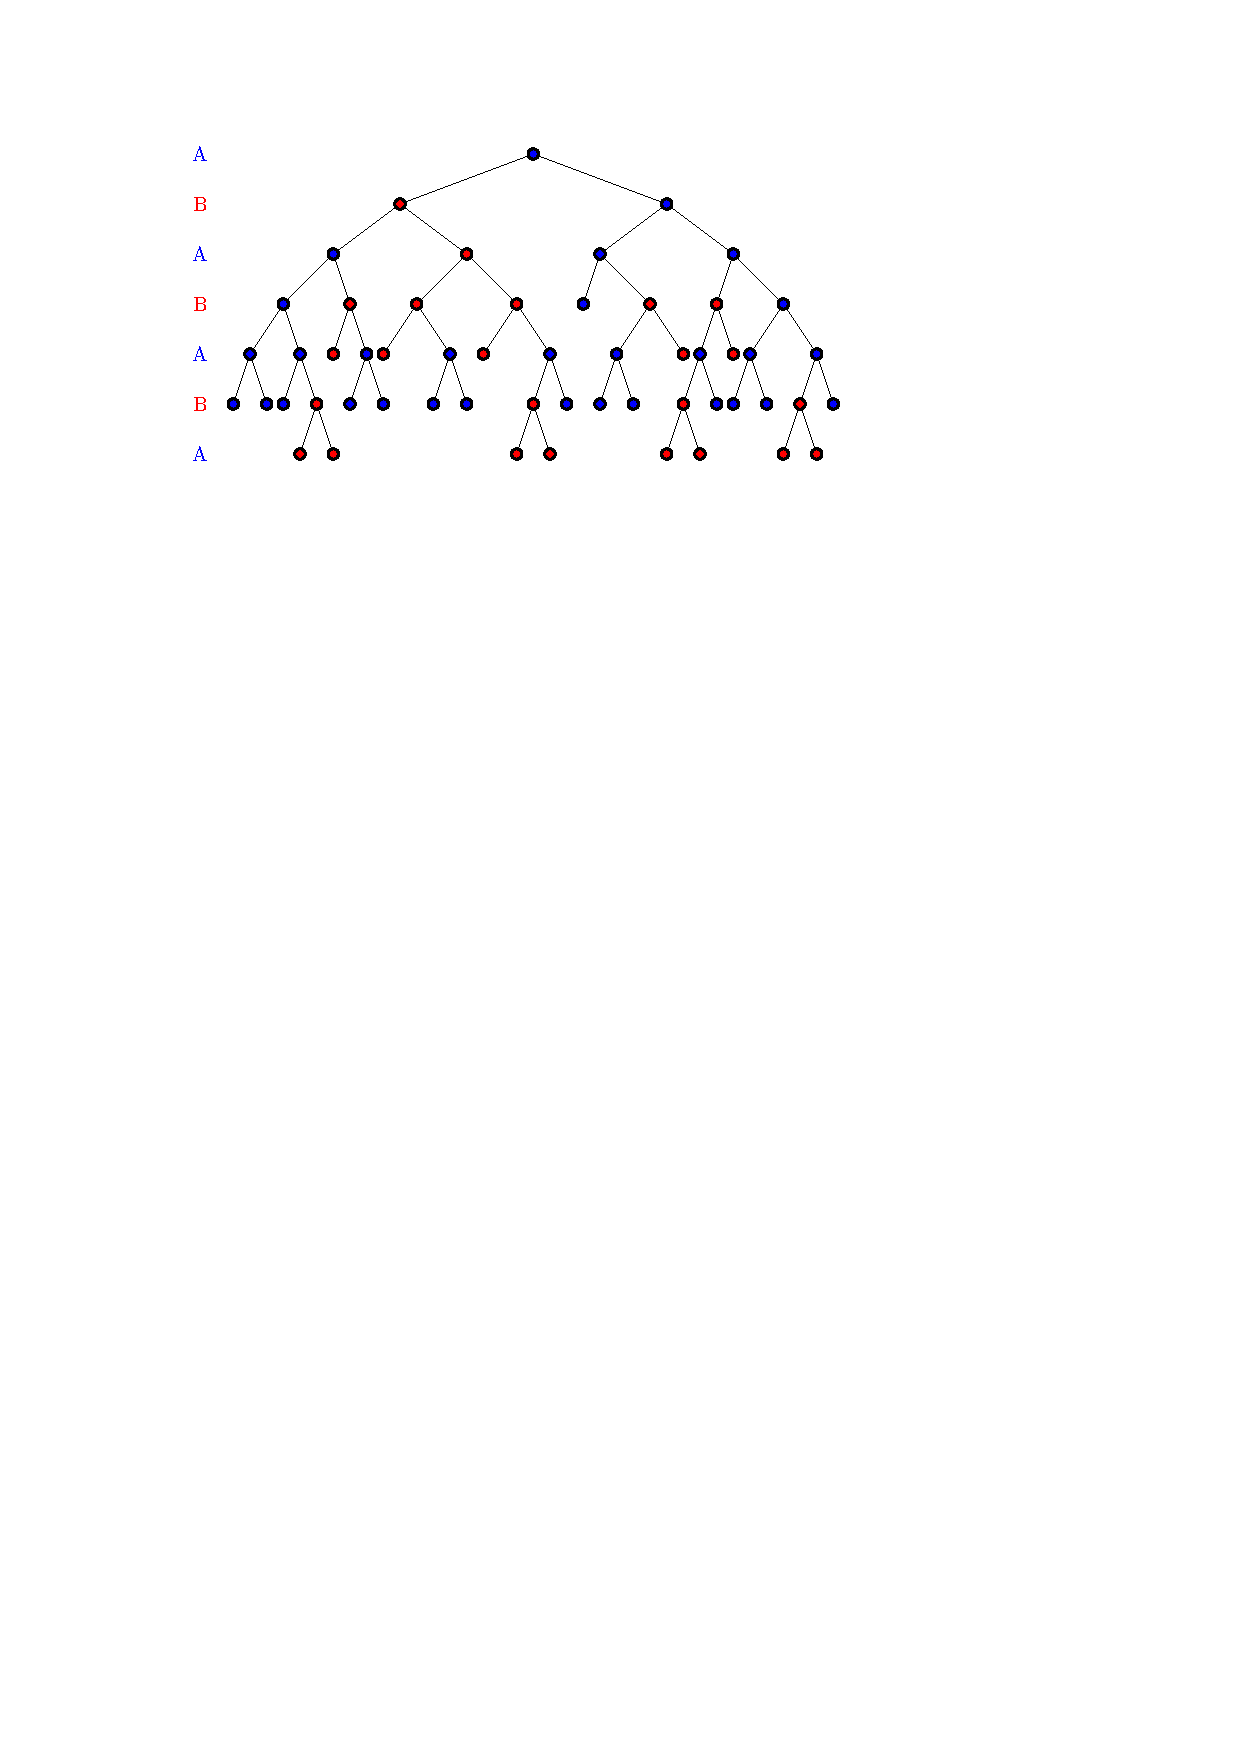
\includegraphics[width=3in]{decisionTree4.pdf}}

%   \vspace{1em}

%   Eventually, we label the entire tree based on when the active player has
%   the option to move into their color or not.
% \end{frame}

% \begin{frame}
%   \centerline{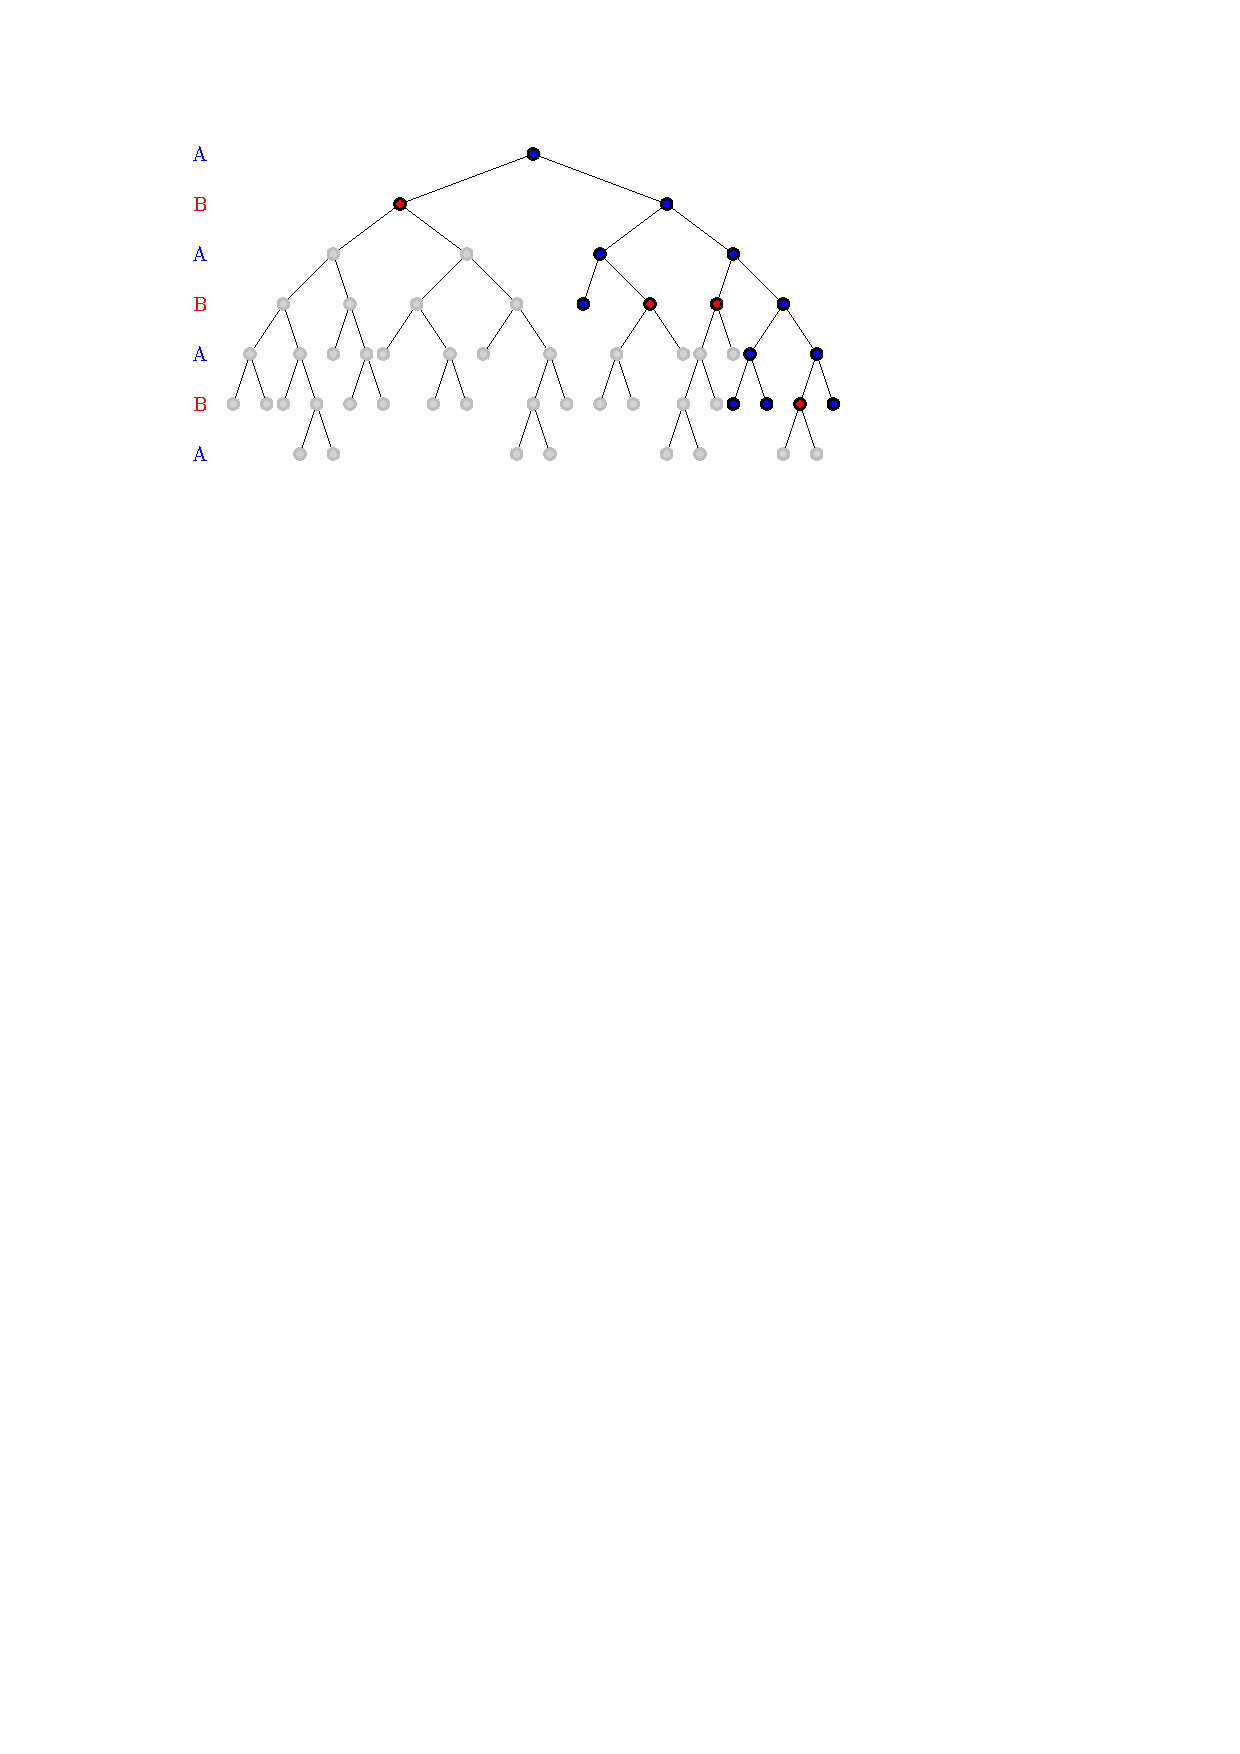
\includegraphics[width=3in]{decisionTree5.pdf}}

%   \vspace{1em}

%   Since the top vertex is blue, $\pl A$ has a winning strategy: always make
%   the choice which leads to another blue vertex.
% \end{frame}

% \section{Infinite Games}

% \subsection{Infinite Games}

% \begin{frame}{Infinite Games}
%   Why do we care so much about determinacy? Why did we define game playthroughs
%   to be infinite sequences?

%   \vpause

%   These topics come into play when considering infinite games.

%   \vpause

%   \begin{definition}
%     A game $G$ is \term{infinite} if there exists a playthrough such that it
%     is still possible for either player to win during every round of the game.
%   \end{definition}
% \end{frame}

% \begin{frame}{How are they played?}
%   Even though a game could never actually be played, we can still construct
%   strategies (functions) and attacks (sequences), and we can compute the
%   result of a game given a strategy and attack.

%   \vpause

%   Put another way, for every infinite game, there is a finite analog of the
%   game which lasts exactly one round: one player chooses a strategy, followed
%   by the opponent choosing an attack based upon it. The result of the infinite
%   game is computed, and that determines the result of the single-round finite
%   game.
% \end{frame}

% \begin{frame}{Determinacy}
%   Like many theorems about infinite mathematical objects, whether infinite
%   games are determined depend on your set-theoretic axioms. Mathematicians who
%   work in foundations often use the Zermelo-Fraenkel (ZF) set theory, which
%   isn't powerful enough to write proofs on the subject.

%   \vpause

%   The \term{Axiom of Determinacy} states that all games which
%   involve (countably) infinite moves are determined: one of the players always
%   can construct a winning strategy.

%   \vpause

%   But the more commonly used \term{Axiom of Choice} can be used to construct
%   a game where if either player fixes a strategy, the other player can always
%   create a counter-attack which defeats it. (See the Banach-Mazur game and
%   Bernstein subsets of the real numbers.)
% \end{frame}

% \subsection{Applications}

% \begin{frame}{Example Game}
%   Let $\<M,W\>$ be \term{Convergence Game $A$} where $M$ is the set of real
%   numbers $\mathbb{R}$, and $A$ is a subset of the real numbers.

%   \vpause

%   Players $\pl A$, $\pl B$ must follow the rule that every real number chosen is
%   strictly between the latest numbers chosen by $\pl A$ and $\pl B$.

%   \vpause

%   The start of a playthrough could be
%     \[
%       \left\<
%         5,
%         \underset{(5<12)}{12},
%         \underset{(5<2\pi<12)}{2\pi},
%         \underset{(2\pi<7<12)}{7},
%         \underset{(2\pi<6.5<7)}{6.5},
%         \dots
%       \right\>
%     \]
% \end{frame}

% \begin{frame}{A Winning Condition}
%   Since there's always infinitely many numbers between every
%   two real numbers, $\pl A$ and $\pl B$ always have legal moves to choose from.

%   \vpause

%   That's why we must add a winning condition: if both players always make legal
%   moves, then $\pl A$ wins if the numbers she chose form a sequence converging
%   to a number in the set $A$, and $\pl B$ wins otherwise.

%   \vpause

%   For example, $\pl A$ won the earlier playthrough if the sequence
%   $\<5,2\pi,6.5,\dots\>$ converges to a number in $A$.
% \end{frame}

% \begin{frame}{Who wins?}
%   \begin{theorem}
%     $\pl B$ has a winning strategy in Convergence Game $A=\{a_0,a_1,\dots\}$
%     (that is, when $A$ is a ``countable'' set).
%   \end{theorem}
% \end{frame}

% \begin{frame}
%   \begin{proof}
%     $\pl B$'s strategy is to take the list of numbers $\{a_0,a_1,\dots\}$,
%     and every turn, $\pl B$ chooses the number furthest to the left of the list
%     which is legal to play.

%     \vpause

%     Then, at the ``end'' of the game, assuming that $\pl A$ also followed the
%     rules, every number in the list $\{a_0,a_1,\dots\}$ is either to the left
%     of one of $\pl A$'s points, or to the right of one of $\pl B$'s points.

%     \vpause

%     Thus, $\pl A$'s points cannot converge to any of the numbers in
%     $\{a_0,a_1,\dots\}$ no matter what attack she attempts.
%   \end{proof}
% \end{frame}

% \begin{frame}{The Application}
%   Using this game, we get a classic set theory result due to Cantor:

%   \vpause

%   \begin{theorem}
%     The real numbers $\mathbb{R}$ cannot be written in a list
%     $\{r_0,r_1,\dots\}$ (they are ``uncountable'').
%   \end{theorem}

%   \begin{proof}
%     Every increasing bounded above sequence converges to a real number
%     (see Cal II). Thus $\pl A$ always wins the Convergence Game $A=\mathbb{R}$.

%     But since $\pl B$ wins if $A$ is a countable set which can be written like
%     $\{a_0,a_1,\dots\}$, we know that $\mathbb{R}$ cannot be countable.
%   \end{proof}
% \end{frame}

\section*{}

\begin{frame}
Questions? Thanks for having me!
\end{frame}


\end{document}


